\documentclass[twoside]{book}

% Packages required by doxygen
\usepackage{fixltx2e}
\usepackage{calc}
\usepackage{doxygen}
\usepackage[export]{adjustbox} % also loads graphicx
\usepackage{graphicx}
\usepackage[utf8]{inputenc}
\usepackage{makeidx}
\usepackage{multicol}
\usepackage{multirow}
\PassOptionsToPackage{warn}{textcomp}
\usepackage{textcomp}
\usepackage[nointegrals]{wasysym}
\usepackage[table]{xcolor}

% NLS support packages
\usepackage[italian]{babel}

% Font selection
\usepackage[T1]{fontenc}
\usepackage[scaled=.90]{helvet}
\usepackage{courier}
\usepackage{amssymb}
\usepackage{sectsty}
\renewcommand{\familydefault}{\sfdefault}
\allsectionsfont{%
  \fontseries{bc}\selectfont%
  \color{darkgray}%
}
\renewcommand{\DoxyLabelFont}{%
  \fontseries{bc}\selectfont%
  \color{darkgray}%
}
\newcommand{\+}{\discretionary{\mbox{\scriptsize$\hookleftarrow$}}{}{}}

% Page & text layout
\usepackage{geometry}
\geometry{%
  a4paper,%
  top=2.5cm,%
  bottom=2.5cm,%
  left=2.5cm,%
  right=2.5cm%
}
\tolerance=750
\hfuzz=15pt
\hbadness=750
\setlength{\emergencystretch}{15pt}
\setlength{\parindent}{0cm}
\setlength{\parskip}{3ex plus 2ex minus 2ex}
\makeatletter
\renewcommand{\paragraph}{%
  \@startsection{paragraph}{4}{0ex}{-1.0ex}{1.0ex}{%
    \normalfont\normalsize\bfseries\SS@parafont%
  }%
}
\renewcommand{\subparagraph}{%
  \@startsection{subparagraph}{5}{0ex}{-1.0ex}{1.0ex}{%
    \normalfont\normalsize\bfseries\SS@subparafont%
  }%
}
\makeatother

% Headers & footers
\usepackage{fancyhdr}
\pagestyle{fancyplain}
\fancyhead[LE]{\fancyplain{}{\bfseries\thepage}}
\fancyhead[CE]{\fancyplain{}{}}
\fancyhead[RE]{\fancyplain{}{\bfseries\leftmark}}
\fancyhead[LO]{\fancyplain{}{\bfseries\rightmark}}
\fancyhead[CO]{\fancyplain{}{}}
\fancyhead[RO]{\fancyplain{}{\bfseries\thepage}}
\fancyfoot[LE]{\fancyplain{}{}}
\fancyfoot[CE]{\fancyplain{}{}}
\fancyfoot[RE]{\fancyplain{}{\bfseries\scriptsize Generato da Doxygen }}
\fancyfoot[LO]{\fancyplain{}{\bfseries\scriptsize Generato da Doxygen }}
\fancyfoot[CO]{\fancyplain{}{}}
\fancyfoot[RO]{\fancyplain{}{}}
\renewcommand{\footrulewidth}{0.4pt}
\renewcommand{\chaptermark}[1]{%
  \markboth{#1}{}%
}
\renewcommand{\sectionmark}[1]{%
  \markright{\thesection\ #1}%
}

% Indices & bibliography
\usepackage{natbib}
\usepackage[titles]{tocloft}
\setcounter{tocdepth}{3}
\setcounter{secnumdepth}{5}
\makeindex

% Hyperlinks (required, but should be loaded last)
\usepackage{ifpdf}
\ifpdf
  \usepackage[pdftex,pagebackref=true]{hyperref}
\else
  \usepackage[ps2pdf,pagebackref=true]{hyperref}
\fi
\hypersetup{%
  colorlinks=true,%
  linkcolor=blue,%
  citecolor=blue,%
  unicode%
}

% Custom commands
\newcommand{\clearemptydoublepage}{%
  \newpage{\pagestyle{empty}\cleardoublepage}%
}

\usepackage{caption}
\captionsetup{labelsep=space,justification=centering,font={bf},singlelinecheck=off,skip=4pt,position=top}

%===== C O N T E N T S =====

\begin{document}

% Titlepage & ToC
\hypersetup{pageanchor=false,
             bookmarksnumbered=true,
             pdfencoding=unicode
            }
\pagenumbering{alph}
\begin{titlepage}
\vspace*{7cm}
\begin{center}%
{\Large Biblioteca \\[1ex]\large 1.\+0 }\\
\vspace*{1cm}
{\large Generato da Doxygen 1.8.14}\\
\end{center}
\end{titlepage}
\clearemptydoublepage
\pagenumbering{roman}
\tableofcontents
\clearemptydoublepage
\pagenumbering{arabic}
\hypersetup{pageanchor=true}

%--- Begin generated contents ---
\chapter{Gestione Simulata di una Biblioteca}
\label{index}\hypertarget{index}{}Questa e\textquotesingle{} una simulazione per il funzionamento di una Biblioteca.~\newline
Tramite il sofware a riga di comando e\textquotesingle{} possibile accedere al servizio secondo tre modalita\textquotesingle{}\+:~\newline
1) \mbox{\hyperlink{class_direttore}{Direttore}} -\/ ha il controllo totale su Libri, Prestiti, Utenti e Addetti~\newline
2) \mbox{\hyperlink{class_addetto}{Addetto}} -\/ rispetto al \mbox{\hyperlink{class_direttore}{Direttore}}, non gestisce gli Addetti e non ha il controllo sull\textquotesingle{}eliminazione di dati~\newline
3) \mbox{\hyperlink{class_utente}{Utente}} -\/ visualizza e ricerca Libri tramite il \mbox{\hyperlink{class_catalogo}{Catalogo}} e controlla i Prestiti da lui effettuati~\newline
\begin{DoxyAuthor}{Autore}
Matteo Pompilio 
\end{DoxyAuthor}
\begin{DoxyVersion}{Versione}
1.\+0 
\end{DoxyVersion}
\begin{DoxyDate}{Data}
18/05/2018 
\end{DoxyDate}

\chapter{Indice della gerarchia}
\section{Gerarchia delle classi}
Questo elenco di ereditarietà è ordinato approssimativamente, ma non completamente, in ordine alfabetico\+:\begin{DoxyCompactList}
\item \contentsline{section}{Catalogo}{\pageref{class_catalogo}}{}
\item \contentsline{section}{Data}{\pageref{class_data}}{}
\item \contentsline{section}{Libro}{\pageref{class_libro}}{}
\item \contentsline{section}{Login}{\pageref{class_login}}{}
\item \contentsline{section}{Persona}{\pageref{class_persona}}{}
\begin{DoxyCompactList}
\item \contentsline{section}{Addetto}{\pageref{class_addetto}}{}
\item \contentsline{section}{Direttore}{\pageref{class_direttore}}{}
\item \contentsline{section}{Utente}{\pageref{class_utente}}{}
\end{DoxyCompactList}
\item \contentsline{section}{Pin}{\pageref{class_pin}}{}
\item \contentsline{section}{Prestito}{\pageref{class_prestito}}{}
\item \contentsline{section}{Registrazione}{\pageref{class_registrazione}}{}
\end{DoxyCompactList}

\chapter{Indice dei tipi composti}
\section{Elenco dei tipi composti}
Queste sono le classi, le struct, le union e le interfacce con una loro breve descrizione\+:\begin{DoxyCompactList}
\item\contentsline{section}{\mbox{\hyperlink{class_addetto}{Addetto}} }{\pageref{class_addetto}}{}
\item\contentsline{section}{\mbox{\hyperlink{class_catalogo}{Catalogo}} }{\pageref{class_catalogo}}{}
\item\contentsline{section}{\mbox{\hyperlink{class_data}{Data}} }{\pageref{class_data}}{}
\item\contentsline{section}{\mbox{\hyperlink{class_direttore}{Direttore}} }{\pageref{class_direttore}}{}
\item\contentsline{section}{\mbox{\hyperlink{class_libro}{Libro}} }{\pageref{class_libro}}{}
\item\contentsline{section}{\mbox{\hyperlink{class_login}{Login}} }{\pageref{class_login}}{}
\item\contentsline{section}{\mbox{\hyperlink{class_persona}{Persona}} }{\pageref{class_persona}}{}
\item\contentsline{section}{\mbox{\hyperlink{class_pin}{Pin}} }{\pageref{class_pin}}{}
\item\contentsline{section}{\mbox{\hyperlink{class_prestito}{Prestito}} }{\pageref{class_prestito}}{}
\item\contentsline{section}{\mbox{\hyperlink{class_registrazione}{Registrazione}} }{\pageref{class_registrazione}}{}
\item\contentsline{section}{\mbox{\hyperlink{class_utente}{Utente}} }{\pageref{class_utente}}{}
\end{DoxyCompactList}

\chapter{Indice dei file}
\section{Elenco dei file}
Questo è un elenco dei file documentati con una loro breve descrizione\+:\begin{DoxyCompactList}
\item\contentsline{section}{\mbox{\hyperlink{classi_8h}{classi.\+h}} \\*Header per la prototipazione delle classi }{\pageref{classi_8h}}{}
\item\contentsline{section}{\mbox{\hyperlink{funzioni_8cpp}{funzioni.\+cpp}} \\*Qua sono implementate tutte le funzioni }{\pageref{funzioni_8cpp}}{}
\item\contentsline{section}{\mbox{\hyperlink{main_8cpp}{main.\+cpp}} \\*Da qui parte il software }{\pageref{main_8cpp}}{}
\end{DoxyCompactList}

\chapter{Documentazione delle classi}
\hypertarget{class_addetto}{}\section{Riferimenti per la classe Addetto}
\label{class_addetto}\index{Addetto@{Addetto}}
Diagramma delle classi per Addetto\begin{figure}[H]
\begin{center}
\leavevmode
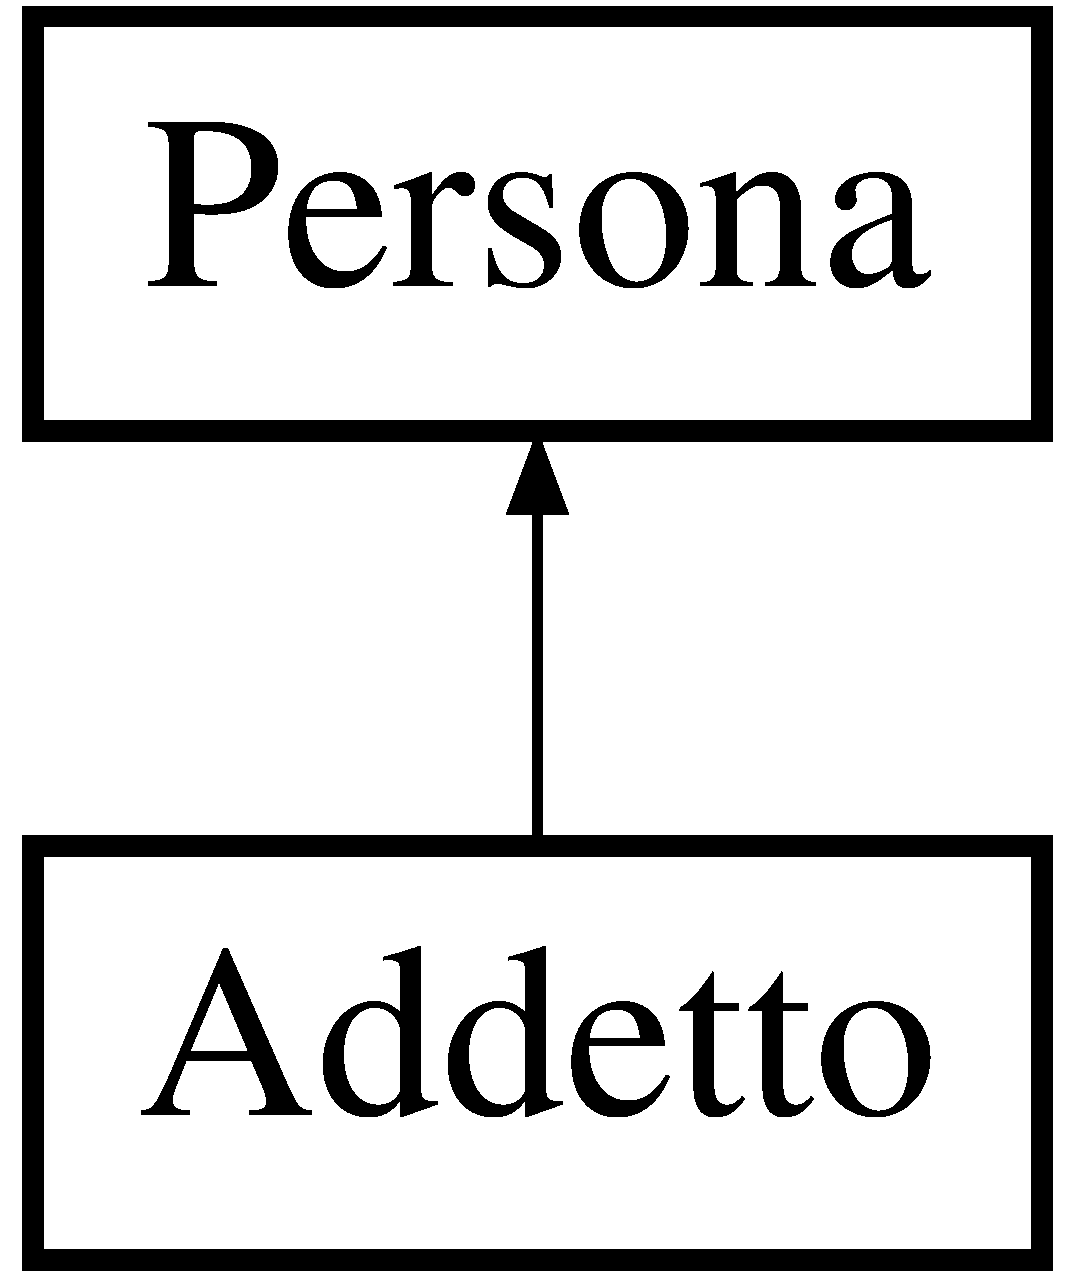
\includegraphics[height=2.000000cm]{class_addetto}
\end{center}
\end{figure}
\subsection*{Membri pubblici}
\begin{DoxyCompactItemize}
\item 
\mbox{\Hypertarget{class_addetto_a6aab9117b8a6f4187e8ef11bf6d3279b}\label{class_addetto_a6aab9117b8a6f4187e8ef11bf6d3279b}} 
\mbox{\hyperlink{class_addetto_a6aab9117b8a6f4187e8ef11bf6d3279b}{Addetto}} (char $\ast$, char $\ast$, char $\ast$)
\begin{DoxyCompactList}\small\item\em Costruttore \mbox{\hyperlink{class_addetto}{Addetto}}. \end{DoxyCompactList}\item 
\mbox{\Hypertarget{class_addetto_ac2edc0ee9e5b3ed99c73ab0a2911ccc9}\label{class_addetto_ac2edc0ee9e5b3ed99c73ab0a2911ccc9}} 
\mbox{\hyperlink{class_addetto_ac2edc0ee9e5b3ed99c73ab0a2911ccc9}{Addetto}} ()
\begin{DoxyCompactList}\small\item\em Costruttore \mbox{\hyperlink{class_addetto}{Addetto}}. \end{DoxyCompactList}\end{DoxyCompactItemize}


La documentazione per questa classe è stata generata a partire dai seguenti file\+:\begin{DoxyCompactItemize}
\item 
\mbox{\hyperlink{classi_8h}{classi.\+h}}\item 
\mbox{\hyperlink{funzioni_8cpp}{funzioni.\+cpp}}\end{DoxyCompactItemize}

\hypertarget{class_catalogo}{}\section{Riferimenti per la classe Catalogo}
\label{class_catalogo}\index{Catalogo@{Catalogo}}
\subsection*{Membri pubblici}
\begin{DoxyCompactItemize}
\item 
\mbox{\hyperlink{class_catalogo_af2d231942828cd6e47bdb17f4215d5d6}{Catalogo}} ()
\begin{DoxyCompactList}\small\item\em Costruttore \mbox{\hyperlink{class_catalogo}{Catalogo}}. \end{DoxyCompactList}\item 
\mbox{\Hypertarget{class_catalogo_af1b86a93a832982c779e34b5ce9dd88b}\label{class_catalogo_af1b86a93a832982c779e34b5ce9dd88b}} 
\mbox{\hyperlink{class_catalogo_af1b86a93a832982c779e34b5ce9dd88b}{$\sim$\+Catalogo}} ()
\begin{DoxyCompactList}\small\item\em Distruttore \mbox{\hyperlink{class_catalogo}{Catalogo}}. \end{DoxyCompactList}\item 
void \mbox{\hyperlink{class_catalogo_a1ba3cde9c46e9d8f5bf6654c7b96647f}{Visualizza\+Catalogo}} ()
\begin{DoxyCompactList}\small\item\em Visualizzatore del \mbox{\hyperlink{class_catalogo}{Catalogo}}. \end{DoxyCompactList}\item 
\mbox{\Hypertarget{class_catalogo_aeaae558ee214dc61944b0a145932fd44}\label{class_catalogo_aeaae558ee214dc61944b0a145932fd44}} 
void \mbox{\hyperlink{class_catalogo_aeaae558ee214dc61944b0a145932fd44}{Update\+Catalogo}} (\mbox{\hyperlink{class_libro}{Libro}} $\ast$)
\begin{DoxyCompactList}\small\item\em Metodo per la modifica di Libri in \mbox{\hyperlink{class_catalogo}{Catalogo}}. \end{DoxyCompactList}\item 
bool \mbox{\hyperlink{class_catalogo_a378e5b182d45ccfba3ace696656cb1d0}{Ricerca\+Libro}} (int $\ast$vett=new int\mbox{[}1000\mbox{]})
\begin{DoxyCompactList}\small\item\em Ricercatore del \mbox{\hyperlink{class_libro}{Libro}}. \end{DoxyCompactList}\end{DoxyCompactItemize}


\subsection{Documentazione dei costruttori e dei distruttori}
\mbox{\Hypertarget{class_catalogo_af2d231942828cd6e47bdb17f4215d5d6}\label{class_catalogo_af2d231942828cd6e47bdb17f4215d5d6}} 
\index{Catalogo@{Catalogo}!Catalogo@{Catalogo}}
\index{Catalogo@{Catalogo}!Catalogo@{Catalogo}}
\subsubsection{\texorpdfstring{Catalogo()}{Catalogo()}}
{\footnotesize\ttfamily Catalogo\+::\+Catalogo (\begin{DoxyParamCaption}{ }\end{DoxyParamCaption})}



Costruttore \mbox{\hyperlink{class_catalogo}{Catalogo}}. 

Provvede ad inserire in Lista Prestiti Scaduti tutti quei Prestiti con \mbox{\hyperlink{class_data}{Data}} di Scadenza $<$= 0. 

\subsection{Documentazione delle funzioni membro}
\mbox{\Hypertarget{class_catalogo_a378e5b182d45ccfba3ace696656cb1d0}\label{class_catalogo_a378e5b182d45ccfba3ace696656cb1d0}} 
\index{Catalogo@{Catalogo}!Ricerca\+Libro@{Ricerca\+Libro}}
\index{Ricerca\+Libro@{Ricerca\+Libro}!Catalogo@{Catalogo}}
\subsubsection{\texorpdfstring{Ricerca\+Libro()}{RicercaLibro()}}
{\footnotesize\ttfamily bool Catalogo\+::\+Ricerca\+Libro (\begin{DoxyParamCaption}\item[{int $\ast$}]{vett = {\ttfamily new~int\mbox{[}1000\mbox{]}} }\end{DoxyParamCaption})}



Ricercatore del \mbox{\hyperlink{class_libro}{Libro}}. 


\begin{DoxyParams}[1]{Parametri}
\mbox{\tt out}  & {\em Conferma} & booleana presenza record in file.\\
\hline
\end{DoxyParams}
Richiede un testo in input, che varra\textquotesingle{} come parola chiave da ricercare in Titolo, Autore, Anno, Codice.~\newline
Restituisce, come indirizzo, un int$\ast$\mbox{[}1000\mbox{]} contenente gli indici dei singoli Libri trovati. \mbox{\Hypertarget{class_catalogo_a1ba3cde9c46e9d8f5bf6654c7b96647f}\label{class_catalogo_a1ba3cde9c46e9d8f5bf6654c7b96647f}} 
\index{Catalogo@{Catalogo}!Visualizza\+Catalogo@{Visualizza\+Catalogo}}
\index{Visualizza\+Catalogo@{Visualizza\+Catalogo}!Catalogo@{Catalogo}}
\subsubsection{\texorpdfstring{Visualizza\+Catalogo()}{VisualizzaCatalogo()}}
{\footnotesize\ttfamily void Catalogo\+::\+Visualizza\+Catalogo (\begin{DoxyParamCaption}{ }\end{DoxyParamCaption})}



Visualizzatore del \mbox{\hyperlink{class_catalogo}{Catalogo}}. 

Mostra la lista dei Libri indicandone\+: Titolo, Autore, Anno, Codice, Disponibilita\textquotesingle{}. 

La documentazione per questa classe è stata generata a partire dai seguenti file\+:\begin{DoxyCompactItemize}
\item 
\mbox{\hyperlink{classi_8h}{classi.\+h}}\item 
\mbox{\hyperlink{funzioni_8cpp}{funzioni.\+cpp}}\end{DoxyCompactItemize}

\hypertarget{class_data}{}\section{Riferimenti per la classe Data}
\label{class_data}\index{Data@{Data}}
\subsection*{Membri pubblici}
\begin{DoxyCompactItemize}
\item 
\mbox{\Hypertarget{class_data_af11f741cb7f587e2e495452a8905a22a}\label{class_data_af11f741cb7f587e2e495452a8905a22a}} 
\mbox{\hyperlink{class_data_af11f741cb7f587e2e495452a8905a22a}{Data}} ()
\begin{DoxyCompactList}\small\item\em Costruttore \mbox{\hyperlink{class_data}{Data}}. \end{DoxyCompactList}\item 
\mbox{\Hypertarget{class_data_aab31956423290f0d62dcca47ab4d16dd}\label{class_data_aab31956423290f0d62dcca47ab4d16dd}} 
\mbox{\hyperlink{class_data_aab31956423290f0d62dcca47ab4d16dd}{$\sim$\+Data}} ()
\begin{DoxyCompactList}\small\item\em Distruttore \mbox{\hyperlink{class_data}{Data}}. \end{DoxyCompactList}\item 
void \mbox{\hyperlink{class_data_a0f77e10131654f6588e1ed935c8b5926}{Set\+Current\+Data\+Ora}} ()
\begin{DoxyCompactList}\small\item\em Setter \mbox{\hyperlink{class_data}{Data}} e Ora correnti. \end{DoxyCompactList}\item 
time\+\_\+t \mbox{\hyperlink{class_data_ab27ede34460ad63d6e3ee2567b3be0d9}{Get\+Data\+Ora}} ()
\begin{DoxyCompactList}\small\item\em Getter \mbox{\hyperlink{class_data}{Data}} e Ora. \end{DoxyCompactList}\item 
time\+\_\+t \mbox{\hyperlink{class_data_aaf254a17c4ad07af79effbd50df887d7}{Get\+Data\+Ora30\+Days}} (time\+\_\+t)
\begin{DoxyCompactList}\small\item\em Getter \mbox{\hyperlink{class_data}{Data}} e Ora sommati di 30 giorni. \end{DoxyCompactList}\item 
time\+\_\+t \mbox{\hyperlink{class_data_a67b1a6fc8bdd632c2bd582206df3c0b7}{Get\+Data\+Ora\+Estesa}} (time\+\_\+t, int)
\begin{DoxyCompactList}\small\item\em Getter \mbox{\hyperlink{class_data}{Data}} e Ora estesi. \end{DoxyCompactList}\end{DoxyCompactItemize}


\subsection{Documentazione delle funzioni membro}
\mbox{\Hypertarget{class_data_ab27ede34460ad63d6e3ee2567b3be0d9}\label{class_data_ab27ede34460ad63d6e3ee2567b3be0d9}} 
\index{Data@{Data}!Get\+Data\+Ora@{Get\+Data\+Ora}}
\index{Get\+Data\+Ora@{Get\+Data\+Ora}!Data@{Data}}
\subsubsection{\texorpdfstring{Get\+Data\+Ora()}{GetDataOra()}}
{\footnotesize\ttfamily time\+\_\+t Data\+::\+Get\+Data\+Ora (\begin{DoxyParamCaption}{ }\end{DoxyParamCaption})}



Getter \mbox{\hyperlink{class_data}{Data}} e Ora. 


\begin{DoxyParams}[1]{Parametri}
\mbox{\tt out}  & {\em time\+\_\+t} & data\+Ora\\
\hline
\end{DoxyParams}
Restituisce \mbox{\hyperlink{class_data}{Data}} e Ora settati mediante la funzione \mbox{\hyperlink{class_data_a0f77e10131654f6588e1ed935c8b5926}{Set\+Current\+Data\+Ora()}}. \mbox{\Hypertarget{class_data_aaf254a17c4ad07af79effbd50df887d7}\label{class_data_aaf254a17c4ad07af79effbd50df887d7}} 
\index{Data@{Data}!Get\+Data\+Ora30\+Days@{Get\+Data\+Ora30\+Days}}
\index{Get\+Data\+Ora30\+Days@{Get\+Data\+Ora30\+Days}!Data@{Data}}
\subsubsection{\texorpdfstring{Get\+Data\+Ora30\+Days()}{GetDataOra30Days()}}
{\footnotesize\ttfamily time\+\_\+t Data\+::\+Get\+Data\+Ora30\+Days (\begin{DoxyParamCaption}\item[{time\+\_\+t}]{data }\end{DoxyParamCaption})}



Getter \mbox{\hyperlink{class_data}{Data}} e Ora sommati di 30 giorni. 


\begin{DoxyParams}[1]{Parametri}
\mbox{\tt out}  & {\em \mbox{\hyperlink{class_data}{Data}}} & e Ora + 30 giorni\\
\hline
\end{DoxyParams}
Restituisce \mbox{\hyperlink{class_data}{Data}} e Ora sommati di 30 giorni al parametro time\+\_\+t in ingresso. \mbox{\Hypertarget{class_data_a67b1a6fc8bdd632c2bd582206df3c0b7}\label{class_data_a67b1a6fc8bdd632c2bd582206df3c0b7}} 
\index{Data@{Data}!Get\+Data\+Ora\+Estesa@{Get\+Data\+Ora\+Estesa}}
\index{Get\+Data\+Ora\+Estesa@{Get\+Data\+Ora\+Estesa}!Data@{Data}}
\subsubsection{\texorpdfstring{Get\+Data\+Ora\+Estesa()}{GetDataOraEstesa()}}
{\footnotesize\ttfamily time\+\_\+t Data\+::\+Get\+Data\+Ora\+Estesa (\begin{DoxyParamCaption}\item[{time\+\_\+t}]{scadenza,  }\item[{int}]{giorni }\end{DoxyParamCaption})}



Getter \mbox{\hyperlink{class_data}{Data}} e Ora estesi. 


\begin{DoxyParams}[1]{Parametri}
\mbox{\tt out}  & {\em \mbox{\hyperlink{class_data}{Data}}} & e Ora + giorni di estensione\\
\hline
\end{DoxyParams}
Restituisce \mbox{\hyperlink{class_data}{Data}} e Ora sommati di \mbox{[}parametro int in ingresso\mbox{]} giorni al parametro time\+\_\+t in ingresso. \mbox{\Hypertarget{class_data_a0f77e10131654f6588e1ed935c8b5926}\label{class_data_a0f77e10131654f6588e1ed935c8b5926}} 
\index{Data@{Data}!Set\+Current\+Data\+Ora@{Set\+Current\+Data\+Ora}}
\index{Set\+Current\+Data\+Ora@{Set\+Current\+Data\+Ora}!Data@{Data}}
\subsubsection{\texorpdfstring{Set\+Current\+Data\+Ora()}{SetCurrentDataOra()}}
{\footnotesize\ttfamily void Data\+::\+Set\+Current\+Data\+Ora (\begin{DoxyParamCaption}{ }\end{DoxyParamCaption})}



Setter \mbox{\hyperlink{class_data}{Data}} e Ora correnti. 

Mediante la funzione time() viene settato un valore time\+\_\+t che contiene \mbox{\hyperlink{class_data}{Data}} e Ora correnti. 

La documentazione per questa classe è stata generata a partire dai seguenti file\+:\begin{DoxyCompactItemize}
\item 
\mbox{\hyperlink{classi_8h}{classi.\+h}}\item 
\mbox{\hyperlink{funzioni_8cpp}{funzioni.\+cpp}}\end{DoxyCompactItemize}

\hypertarget{class_direttore}{}\section{Riferimenti per la classe Direttore}
\label{class_direttore}\index{Direttore@{Direttore}}
Diagramma delle classi per Direttore\begin{figure}[H]
\begin{center}
\leavevmode
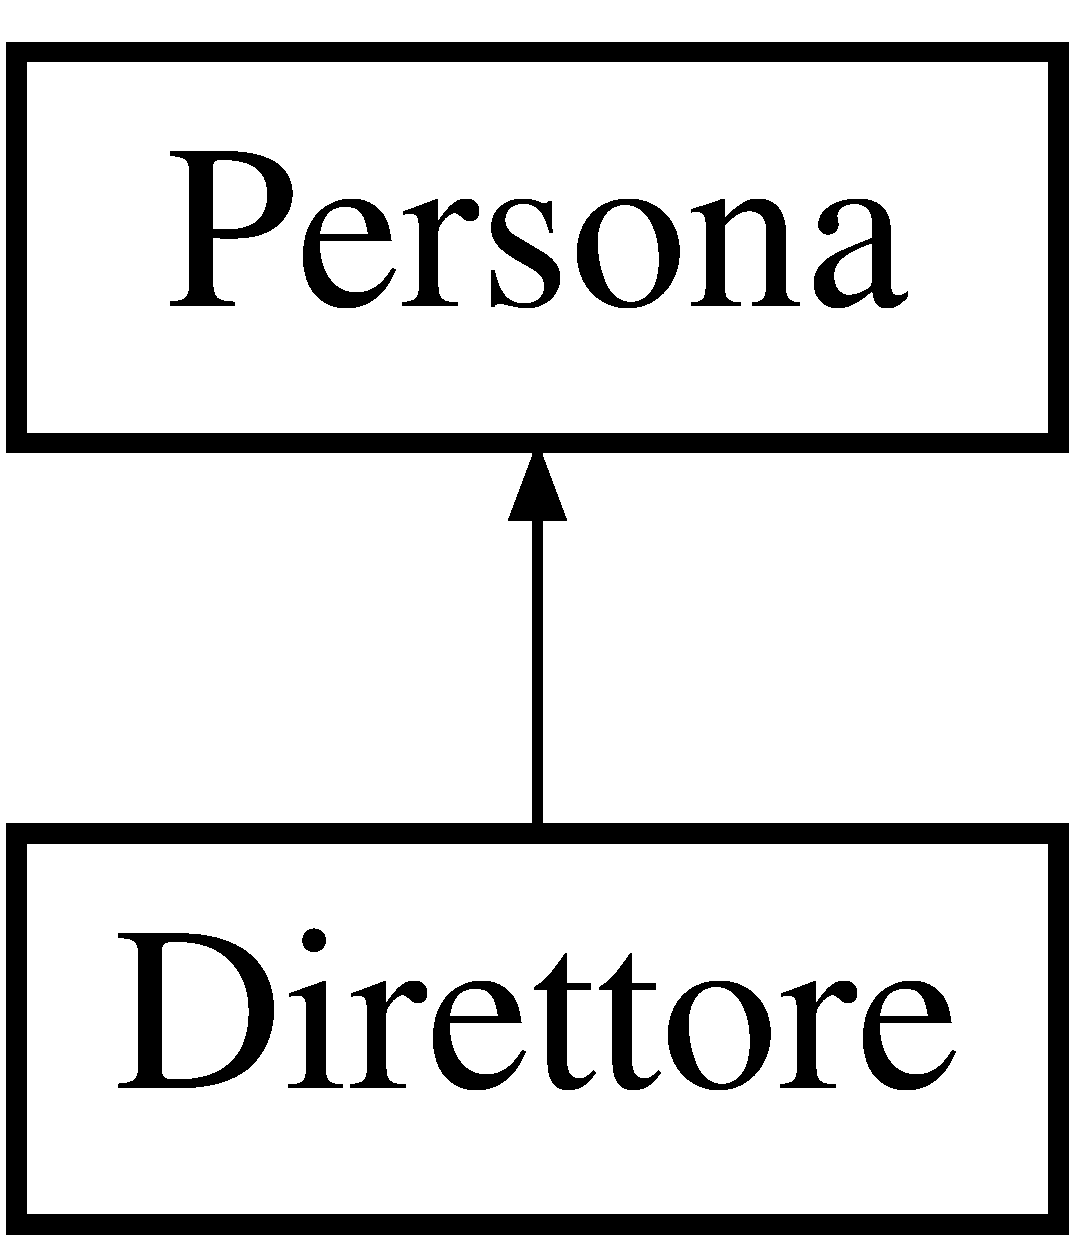
\includegraphics[height=2.000000cm]{class_direttore}
\end{center}
\end{figure}
\subsection*{Membri pubblici}
\begin{DoxyCompactItemize}
\item 
\mbox{\Hypertarget{class_direttore_aa4f96257cc680cb6bab2f288f9c36c45}\label{class_direttore_aa4f96257cc680cb6bab2f288f9c36c45}} 
\mbox{\hyperlink{class_direttore_aa4f96257cc680cb6bab2f288f9c36c45}{Direttore}} (char $\ast$, char $\ast$, char $\ast$)
\begin{DoxyCompactList}\small\item\em Costruttore \mbox{\hyperlink{class_direttore}{Direttore}}. \end{DoxyCompactList}\item 
\mbox{\Hypertarget{class_direttore_a2454c9f9e9c608c4d11ee706e9a0b84e}\label{class_direttore_a2454c9f9e9c608c4d11ee706e9a0b84e}} 
\mbox{\hyperlink{class_direttore_a2454c9f9e9c608c4d11ee706e9a0b84e}{Direttore}} ()
\begin{DoxyCompactList}\small\item\em Costruttore \mbox{\hyperlink{class_direttore}{Direttore}}. \end{DoxyCompactList}\item 
void \mbox{\hyperlink{class_direttore_a129587a726e0980dc6873c1bfdc815b7}{View\+Lista\+Addetti}} ()
\begin{DoxyCompactList}\small\item\em Visualizzatore della Lista Addetti. \end{DoxyCompactList}\item 
bool \mbox{\hyperlink{class_direttore_af105ccdec38de04af05540a4abb318b6}{Ricerca\+Addetto}} (int $\ast$vett=new int\mbox{[}1000\mbox{]})
\begin{DoxyCompactList}\small\item\em Ricercatore dell\textquotesingle{}\mbox{\hyperlink{class_addetto}{Addetto}}. \end{DoxyCompactList}\item 
void \mbox{\hyperlink{class_direttore_ae68ff6aa5d4ef52bb2d13fe6196be098}{Registrazione\+Addetto}} ()
\begin{DoxyCompactList}\small\item\em Registratore dell\textquotesingle{}\mbox{\hyperlink{class_addetto}{Addetto}}. \end{DoxyCompactList}\item 
void \mbox{\hyperlink{class_direttore_a9516369e5ecf44407d616503274b24e0}{Modifica\+Prestito}} ()
\begin{DoxyCompactList}\small\item\em Modificatore del \mbox{\hyperlink{class_prestito}{Prestito}}. \end{DoxyCompactList}\item 
void \mbox{\hyperlink{class_direttore_a60fad939a27c6757cbd1178342dd1ee4}{Modifica\+Addetto}} ()
\begin{DoxyCompactList}\small\item\em Modificatore dell\textquotesingle{}\mbox{\hyperlink{class_addetto}{Addetto}}. \end{DoxyCompactList}\item 
void \mbox{\hyperlink{class_direttore_a123715efe14406e729ad049538bd6ef7}{Eliminazione\+Libro}} ()
\begin{DoxyCompactList}\small\item\em Eliminatore del \mbox{\hyperlink{class_libro}{Libro}}. \end{DoxyCompactList}\item 
void \mbox{\hyperlink{class_direttore_a244e9b158142cee49c48c00c44a44f2c}{Eliminazione\+Prestito}} ()
\begin{DoxyCompactList}\small\item\em Eliminatore del \mbox{\hyperlink{class_prestito}{Prestito}}. \end{DoxyCompactList}\item 
void \mbox{\hyperlink{class_direttore_a9af311211927da3e2e34ddefe0506e99}{Eliminazione\+In\+Lista\+Prestiti}} (char $\ast$username=\char`\"{}\char`\"{}, char $\ast$codice\+Libro=\char`\"{}\char`\"{})
\begin{DoxyCompactList}\small\item\em Eliminatore del \mbox{\hyperlink{class_prestito}{Prestito}} in Lista Prestiti Richiesti. \end{DoxyCompactList}\item 
void \mbox{\hyperlink{class_direttore_a404a98bb33a0437aa605f2a3c35a2db4}{Eliminazione\+In\+Lista\+Prestiti\+In\+Corso}} (char $\ast$username=\char`\"{}\char`\"{}, char $\ast$codice\+Libro=\char`\"{}\char`\"{})
\begin{DoxyCompactList}\small\item\em Eliminatore del \mbox{\hyperlink{class_prestito}{Prestito}} in Lista Prestiti In Corso. \end{DoxyCompactList}\item 
void \mbox{\hyperlink{class_direttore_acc0f5fcd26f5adbd5ea5c3f54f01b34a}{Eliminazione\+Utente}} ()
\begin{DoxyCompactList}\small\item\em Eliminatore dell\textquotesingle{}\mbox{\hyperlink{class_utente}{Utente}}. \end{DoxyCompactList}\item 
void \mbox{\hyperlink{class_direttore_a32293a43bb28f02eb543090d828f7738}{Eliminazione\+Addetto}} ()
\begin{DoxyCompactList}\small\item\em Eliminatore dell\textquotesingle{}\mbox{\hyperlink{class_addetto}{Addetto}}. \end{DoxyCompactList}\end{DoxyCompactItemize}


\subsection{Documentazione delle funzioni membro}
\mbox{\Hypertarget{class_direttore_a32293a43bb28f02eb543090d828f7738}\label{class_direttore_a32293a43bb28f02eb543090d828f7738}} 
\index{Direttore@{Direttore}!Eliminazione\+Addetto@{Eliminazione\+Addetto}}
\index{Eliminazione\+Addetto@{Eliminazione\+Addetto}!Direttore@{Direttore}}
\subsubsection{\texorpdfstring{Eliminazione\+Addetto()}{EliminazioneAddetto()}}
{\footnotesize\ttfamily void Direttore\+::\+Eliminazione\+Addetto (\begin{DoxyParamCaption}{ }\end{DoxyParamCaption})}



Eliminatore dell\textquotesingle{}\mbox{\hyperlink{class_addetto}{Addetto}}. 

Richiamando la funzione \mbox{\hyperlink{class_direttore_af105ccdec38de04af05540a4abb318b6}{Ricerca\+Addetto()}} ne chiede la selezione dell\textquotesingle{}\mbox{\hyperlink{class_addetto}{Addetto}} e, una volta selezionato,~\newline
provvede all\textquotesingle{}eliminazione, eseguita creando un file temporaneo che verra\textquotesingle{} poi rinominato. \mbox{\Hypertarget{class_direttore_a9af311211927da3e2e34ddefe0506e99}\label{class_direttore_a9af311211927da3e2e34ddefe0506e99}} 
\index{Direttore@{Direttore}!Eliminazione\+In\+Lista\+Prestiti@{Eliminazione\+In\+Lista\+Prestiti}}
\index{Eliminazione\+In\+Lista\+Prestiti@{Eliminazione\+In\+Lista\+Prestiti}!Direttore@{Direttore}}
\subsubsection{\texorpdfstring{Eliminazione\+In\+Lista\+Prestiti()}{EliminazioneInListaPrestiti()}}
{\footnotesize\ttfamily void Direttore\+::\+Eliminazione\+In\+Lista\+Prestiti (\begin{DoxyParamCaption}\item[{char $\ast$}]{username = {\ttfamily \char`\"{}\char`\"{}},  }\item[{char $\ast$}]{codice\+Libro = {\ttfamily \char`\"{}\char`\"{}} }\end{DoxyParamCaption})}



Eliminatore del \mbox{\hyperlink{class_prestito}{Prestito}} in Lista Prestiti Richiesti. 

Metodo richiamato unicamente dalla funzione \mbox{\hyperlink{class_direttore_a244e9b158142cee49c48c00c44a44f2c}{Eliminazione\+Prestito()}}. \mbox{\Hypertarget{class_direttore_a404a98bb33a0437aa605f2a3c35a2db4}\label{class_direttore_a404a98bb33a0437aa605f2a3c35a2db4}} 
\index{Direttore@{Direttore}!Eliminazione\+In\+Lista\+Prestiti\+In\+Corso@{Eliminazione\+In\+Lista\+Prestiti\+In\+Corso}}
\index{Eliminazione\+In\+Lista\+Prestiti\+In\+Corso@{Eliminazione\+In\+Lista\+Prestiti\+In\+Corso}!Direttore@{Direttore}}
\subsubsection{\texorpdfstring{Eliminazione\+In\+Lista\+Prestiti\+In\+Corso()}{EliminazioneInListaPrestitiInCorso()}}
{\footnotesize\ttfamily void Direttore\+::\+Eliminazione\+In\+Lista\+Prestiti\+In\+Corso (\begin{DoxyParamCaption}\item[{char $\ast$}]{username = {\ttfamily \char`\"{}\char`\"{}},  }\item[{char $\ast$}]{codice\+Libro = {\ttfamily \char`\"{}\char`\"{}} }\end{DoxyParamCaption})}



Eliminatore del \mbox{\hyperlink{class_prestito}{Prestito}} in Lista Prestiti In Corso. 

Metodo richiamato unicamente dalla funzione \mbox{\hyperlink{class_direttore_a244e9b158142cee49c48c00c44a44f2c}{Eliminazione\+Prestito()}}. \mbox{\Hypertarget{class_direttore_a123715efe14406e729ad049538bd6ef7}\label{class_direttore_a123715efe14406e729ad049538bd6ef7}} 
\index{Direttore@{Direttore}!Eliminazione\+Libro@{Eliminazione\+Libro}}
\index{Eliminazione\+Libro@{Eliminazione\+Libro}!Direttore@{Direttore}}
\subsubsection{\texorpdfstring{Eliminazione\+Libro()}{EliminazioneLibro()}}
{\footnotesize\ttfamily void Direttore\+::\+Eliminazione\+Libro (\begin{DoxyParamCaption}{ }\end{DoxyParamCaption})}



Eliminatore del \mbox{\hyperlink{class_libro}{Libro}}. 

Richiamando la funzione Ricerca\+Libro() ne chiede la selezione del \mbox{\hyperlink{class_libro}{Libro}} e, una volta selezionato,~\newline
provvede all\textquotesingle{}eliminazione, eseguita creando un file temporaneo che verra\textquotesingle{} poi rinominato. \mbox{\Hypertarget{class_direttore_a244e9b158142cee49c48c00c44a44f2c}\label{class_direttore_a244e9b158142cee49c48c00c44a44f2c}} 
\index{Direttore@{Direttore}!Eliminazione\+Prestito@{Eliminazione\+Prestito}}
\index{Eliminazione\+Prestito@{Eliminazione\+Prestito}!Direttore@{Direttore}}
\subsubsection{\texorpdfstring{Eliminazione\+Prestito()}{EliminazionePrestito()}}
{\footnotesize\ttfamily void Direttore\+::\+Eliminazione\+Prestito (\begin{DoxyParamCaption}{ }\end{DoxyParamCaption})}



Eliminatore del \mbox{\hyperlink{class_prestito}{Prestito}}. 

Richiamando la funzione \mbox{\hyperlink{class_persona_ab06e2688ff0eb5c51177a44d33232070}{Ricerca\+Prestito()}} ne chiede la selezione del \mbox{\hyperlink{class_prestito}{Prestito}} e, una volta selezionato,~\newline
provvede all\textquotesingle{}eliminazione, eseguita creando un file temporaneo che verra\textquotesingle{} poi rinominato. \mbox{\Hypertarget{class_direttore_acc0f5fcd26f5adbd5ea5c3f54f01b34a}\label{class_direttore_acc0f5fcd26f5adbd5ea5c3f54f01b34a}} 
\index{Direttore@{Direttore}!Eliminazione\+Utente@{Eliminazione\+Utente}}
\index{Eliminazione\+Utente@{Eliminazione\+Utente}!Direttore@{Direttore}}
\subsubsection{\texorpdfstring{Eliminazione\+Utente()}{EliminazioneUtente()}}
{\footnotesize\ttfamily void Direttore\+::\+Eliminazione\+Utente (\begin{DoxyParamCaption}{ }\end{DoxyParamCaption})}



Eliminatore dell\textquotesingle{}\mbox{\hyperlink{class_utente}{Utente}}. 

Richiamando la funzione \mbox{\hyperlink{class_persona_a11bc0159627eb83be83b00c56ff1a3f9}{Ricerca\+Utente()}} ne chiede la selezione dell\textquotesingle{}\mbox{\hyperlink{class_utente}{Utente}} e, una volta selezionato,~\newline
provvede all\textquotesingle{}eliminazione, eseguita creando un file temporaneo che verra\textquotesingle{} poi rinominato. \mbox{\Hypertarget{class_direttore_a60fad939a27c6757cbd1178342dd1ee4}\label{class_direttore_a60fad939a27c6757cbd1178342dd1ee4}} 
\index{Direttore@{Direttore}!Modifica\+Addetto@{Modifica\+Addetto}}
\index{Modifica\+Addetto@{Modifica\+Addetto}!Direttore@{Direttore}}
\subsubsection{\texorpdfstring{Modifica\+Addetto()}{ModificaAddetto()}}
{\footnotesize\ttfamily void Direttore\+::\+Modifica\+Addetto (\begin{DoxyParamCaption}{ }\end{DoxyParamCaption})}



Modificatore dell\textquotesingle{}\mbox{\hyperlink{class_addetto}{Addetto}}. 

Richiamando la funzione \mbox{\hyperlink{class_direttore_af105ccdec38de04af05540a4abb318b6}{Ricerca\+Addetto()}} ne chiede la selezione dell\textquotesingle{}\mbox{\hyperlink{class_addetto}{Addetto}} e, una volta selezionato,~\newline
elenca i parametri che si vogliono modificare, a scelta tra Nome, Cognome, \mbox{\hyperlink{class_pin}{Pin}}.~\newline
La modifica avviene sia nella Lista Addetti, sia nella Lista Prestiti Scaduti, In Corso e Richiesti. \mbox{\Hypertarget{class_direttore_a9516369e5ecf44407d616503274b24e0}\label{class_direttore_a9516369e5ecf44407d616503274b24e0}} 
\index{Direttore@{Direttore}!Modifica\+Prestito@{Modifica\+Prestito}}
\index{Modifica\+Prestito@{Modifica\+Prestito}!Direttore@{Direttore}}
\subsubsection{\texorpdfstring{Modifica\+Prestito()}{ModificaPrestito()}}
{\footnotesize\ttfamily void Direttore\+::\+Modifica\+Prestito (\begin{DoxyParamCaption}{ }\end{DoxyParamCaption})}



Modificatore del \mbox{\hyperlink{class_prestito}{Prestito}}. 

Richiamando la funzione \mbox{\hyperlink{class_persona_ab06e2688ff0eb5c51177a44d33232070}{Ricerca\+Prestito()}} ne chiede la selezione del \mbox{\hyperlink{class_prestito}{Prestito}} e, una volta selezionato,~\newline
chiede al solo \mbox{\hyperlink{class_direttore}{Direttore}} il numero di giorni da concedere al \mbox{\hyperlink{class_prestito}{Prestito}}, da un minimo di 30 fino a -\/30.~\newline
La modifica avviene in Lista Prestiti In Corso, solamente se il \mbox{\hyperlink{class_prestito}{Prestito}} non � ancora scaduto. \mbox{\Hypertarget{class_direttore_ae68ff6aa5d4ef52bb2d13fe6196be098}\label{class_direttore_ae68ff6aa5d4ef52bb2d13fe6196be098}} 
\index{Direttore@{Direttore}!Registrazione\+Addetto@{Registrazione\+Addetto}}
\index{Registrazione\+Addetto@{Registrazione\+Addetto}!Direttore@{Direttore}}
\subsubsection{\texorpdfstring{Registrazione\+Addetto()}{RegistrazioneAddetto()}}
{\footnotesize\ttfamily void Direttore\+::\+Registrazione\+Addetto (\begin{DoxyParamCaption}{ }\end{DoxyParamCaption})}



Registratore dell\textquotesingle{}\mbox{\hyperlink{class_addetto}{Addetto}}. 

Richiede Nome e Cognome da tastiera e fornisce il relativo \mbox{\hyperlink{class_pin}{Pin}} generato automaticamente. \mbox{\Hypertarget{class_direttore_af105ccdec38de04af05540a4abb318b6}\label{class_direttore_af105ccdec38de04af05540a4abb318b6}} 
\index{Direttore@{Direttore}!Ricerca\+Addetto@{Ricerca\+Addetto}}
\index{Ricerca\+Addetto@{Ricerca\+Addetto}!Direttore@{Direttore}}
\subsubsection{\texorpdfstring{Ricerca\+Addetto()}{RicercaAddetto()}}
{\footnotesize\ttfamily bool Direttore\+::\+Ricerca\+Addetto (\begin{DoxyParamCaption}\item[{int $\ast$}]{vett = {\ttfamily new~int\mbox{[}1000\mbox{]}} }\end{DoxyParamCaption})}



Ricercatore dell\textquotesingle{}\mbox{\hyperlink{class_addetto}{Addetto}}. 


\begin{DoxyParams}[1]{Parametri}
\mbox{\tt out}  & {\em Conferma} & booleana presenza record in file.\\
\hline
\end{DoxyParams}
Richiede un testo in input, che varra\textquotesingle{} come parola chiave da ricercare in Nome, Cognome, \mbox{\hyperlink{class_pin}{Pin}}.~\newline
Restituisce, come indirizzo, un int$\ast$\mbox{[}1000\mbox{]} contenente gli indici dei singoli Addetti trovati. \mbox{\Hypertarget{class_direttore_a129587a726e0980dc6873c1bfdc815b7}\label{class_direttore_a129587a726e0980dc6873c1bfdc815b7}} 
\index{Direttore@{Direttore}!View\+Lista\+Addetti@{View\+Lista\+Addetti}}
\index{View\+Lista\+Addetti@{View\+Lista\+Addetti}!Direttore@{Direttore}}
\subsubsection{\texorpdfstring{View\+Lista\+Addetti()}{ViewListaAddetti()}}
{\footnotesize\ttfamily void Direttore\+::\+View\+Lista\+Addetti (\begin{DoxyParamCaption}{ }\end{DoxyParamCaption})}



Visualizzatore della Lista Addetti. 

Mostra la lista degli Addetti indicandone\+: Nome, Cognome, \mbox{\hyperlink{class_pin}{Pin}}, \mbox{\hyperlink{class_data}{Data}} \mbox{\hyperlink{class_registrazione}{Registrazione}}. 

La documentazione per questa classe è stata generata a partire dai seguenti file\+:\begin{DoxyCompactItemize}
\item 
\mbox{\hyperlink{classi_8h}{classi.\+h}}\item 
\mbox{\hyperlink{funzioni_8cpp}{funzioni.\+cpp}}\end{DoxyCompactItemize}

\hypertarget{class_libro}{}\section{Riferimenti per la classe Libro}
\label{class_libro}\index{Libro@{Libro}}
\subsection*{Membri pubblici}
\begin{DoxyCompactItemize}
\item 
\mbox{\hyperlink{class_libro_a3c8b61b4e44a208cf98b088cd52d22f9}{Libro}} (char $\ast$, char $\ast$, char $\ast$, char $\ast$, bool cod=true)
\begin{DoxyCompactList}\small\item\em Costruttore \mbox{\hyperlink{class_libro}{Libro}}. \end{DoxyCompactList}\item 
\mbox{\Hypertarget{class_libro_a9892c534a717676fdd96b48bb2e0f8bc}\label{class_libro_a9892c534a717676fdd96b48bb2e0f8bc}} 
\mbox{\hyperlink{class_libro_a9892c534a717676fdd96b48bb2e0f8bc}{Libro}} ()
\begin{DoxyCompactList}\small\item\em Costruttore \mbox{\hyperlink{class_libro}{Libro}}. \end{DoxyCompactList}\item 
\mbox{\Hypertarget{class_libro_ab8e4fbae43d4cb308d61ebbadf7dd774}\label{class_libro_ab8e4fbae43d4cb308d61ebbadf7dd774}} 
\mbox{\hyperlink{class_libro_ab8e4fbae43d4cb308d61ebbadf7dd774}{$\sim$\+Libro}} ()
\begin{DoxyCompactList}\small\item\em Distruttore \mbox{\hyperlink{class_libro}{Libro}}. \end{DoxyCompactList}\item 
void \mbox{\hyperlink{class_libro_a0f633fe9a079f98bd34adc1acaa528bb}{Set\+Informazioni}} (char $\ast$, char $\ast$, char $\ast$, char $\ast$, char $\ast$)
\begin{DoxyCompactList}\small\item\em Setter delle credenziali. \end{DoxyCompactList}\item 
void \mbox{\hyperlink{class_libro_a5fd77c4629c2071bf74c8292acc4e11f}{Write}} (\mbox{\hyperlink{class_libro}{Libro}} $\ast$)
\begin{DoxyCompactList}\small\item\em Writer per il nuovo \mbox{\hyperlink{class_libro}{Libro}}. \end{DoxyCompactList}\item 
char $\ast$ \mbox{\hyperlink{class_libro_a150113fad867b05e611f842d49240cbb}{Get\+Titolo}} ()
\begin{DoxyCompactList}\small\item\em Getter per il Titolo. \end{DoxyCompactList}\item 
char $\ast$ \mbox{\hyperlink{class_libro_a8bdd6591dc3b2fd55d1b05f342c66246}{Get\+Autore}} ()
\begin{DoxyCompactList}\small\item\em Getter per l\textquotesingle{}Autore. \end{DoxyCompactList}\item 
char $\ast$ \mbox{\hyperlink{class_libro_af3cc0eebf7a7fc829d7cd7706654cc5c}{Get\+Anno}} ()
\begin{DoxyCompactList}\small\item\em Getter per l\textquotesingle{}Anno. \end{DoxyCompactList}\item 
char $\ast$ \mbox{\hyperlink{class_libro_aee474bbbefdf6a552a24518db05bb97e}{Get\+Codice}} ()
\begin{DoxyCompactList}\small\item\em Getter per il Codice. \end{DoxyCompactList}\item 
\mbox{\Hypertarget{class_libro_ac86f412ccded7666efcf9e75503cfe6c}\label{class_libro_ac86f412ccded7666efcf9e75503cfe6c}} 
void \mbox{\hyperlink{class_libro_ac86f412ccded7666efcf9e75503cfe6c}{Set\+Codice}} (char $\ast$)
\begin{DoxyCompactList}\small\item\em Setter per il Codice. \end{DoxyCompactList}\item 
char $\ast$ \mbox{\hyperlink{class_libro_af8867b8219d6142b33fa2dd7b6f2d0b7}{Get\+Disponibilita}} ()
\begin{DoxyCompactList}\small\item\em Getter per la Disponibilita. \end{DoxyCompactList}\item 
\mbox{\Hypertarget{class_libro_a781639a31b54c34cb43896a25811b5f3}\label{class_libro_a781639a31b54c34cb43896a25811b5f3}} 
void \mbox{\hyperlink{class_libro_a781639a31b54c34cb43896a25811b5f3}{Set\+Disponibilita}} (char $\ast$)
\begin{DoxyCompactList}\small\item\em Setter per la Disponibilita. \end{DoxyCompactList}\end{DoxyCompactItemize}


\subsection{Documentazione dei costruttori e dei distruttori}
\mbox{\Hypertarget{class_libro_a3c8b61b4e44a208cf98b088cd52d22f9}\label{class_libro_a3c8b61b4e44a208cf98b088cd52d22f9}} 
\index{Libro@{Libro}!Libro@{Libro}}
\index{Libro@{Libro}!Libro@{Libro}}
\subsubsection{\texorpdfstring{Libro()}{Libro()}}
{\footnotesize\ttfamily Libro\+::\+Libro (\begin{DoxyParamCaption}\item[{char $\ast$}]{titolo,  }\item[{char $\ast$}]{autore,  }\item[{char $\ast$}]{anno,  }\item[{char $\ast$}]{disponibilita,  }\item[{bool}]{cod = {\ttfamily true} }\end{DoxyParamCaption})}



Costruttore \mbox{\hyperlink{class_libro}{Libro}}. 

Richiede 4 parametri in entrata\+: Titolo, Autore, Anno, Disponibilita.~\newline
In pi� se richiamato con valore booleano settato true (essendo parametro di default), provvede a generare~\newline
un nuovo Codice, calcolato mediante l\textquotesingle{}incremento di un contatore stampato su file binario, riscrivendolo aggiornato. 

\subsection{Documentazione delle funzioni membro}
\mbox{\Hypertarget{class_libro_af3cc0eebf7a7fc829d7cd7706654cc5c}\label{class_libro_af3cc0eebf7a7fc829d7cd7706654cc5c}} 
\index{Libro@{Libro}!Get\+Anno@{Get\+Anno}}
\index{Get\+Anno@{Get\+Anno}!Libro@{Libro}}
\subsubsection{\texorpdfstring{Get\+Anno()}{GetAnno()}}
{\footnotesize\ttfamily char $\ast$ Libro\+::\+Get\+Anno (\begin{DoxyParamCaption}{ }\end{DoxyParamCaption})}



Getter per l\textquotesingle{}Anno. 


\begin{DoxyParams}[1]{Parametri}
\mbox{\tt out}  & {\em char$\ast$} & anno \\
\hline
\end{DoxyParams}
\mbox{\Hypertarget{class_libro_a8bdd6591dc3b2fd55d1b05f342c66246}\label{class_libro_a8bdd6591dc3b2fd55d1b05f342c66246}} 
\index{Libro@{Libro}!Get\+Autore@{Get\+Autore}}
\index{Get\+Autore@{Get\+Autore}!Libro@{Libro}}
\subsubsection{\texorpdfstring{Get\+Autore()}{GetAutore()}}
{\footnotesize\ttfamily char $\ast$ Libro\+::\+Get\+Autore (\begin{DoxyParamCaption}{ }\end{DoxyParamCaption})}



Getter per l\textquotesingle{}Autore. 


\begin{DoxyParams}[1]{Parametri}
\mbox{\tt out}  & {\em char$\ast$} & autore \\
\hline
\end{DoxyParams}
\mbox{\Hypertarget{class_libro_aee474bbbefdf6a552a24518db05bb97e}\label{class_libro_aee474bbbefdf6a552a24518db05bb97e}} 
\index{Libro@{Libro}!Get\+Codice@{Get\+Codice}}
\index{Get\+Codice@{Get\+Codice}!Libro@{Libro}}
\subsubsection{\texorpdfstring{Get\+Codice()}{GetCodice()}}
{\footnotesize\ttfamily char $\ast$ Libro\+::\+Get\+Codice (\begin{DoxyParamCaption}{ }\end{DoxyParamCaption})}



Getter per il Codice. 


\begin{DoxyParams}[1]{Parametri}
\mbox{\tt out}  & {\em char$\ast$} & codice \\
\hline
\end{DoxyParams}
\mbox{\Hypertarget{class_libro_af8867b8219d6142b33fa2dd7b6f2d0b7}\label{class_libro_af8867b8219d6142b33fa2dd7b6f2d0b7}} 
\index{Libro@{Libro}!Get\+Disponibilita@{Get\+Disponibilita}}
\index{Get\+Disponibilita@{Get\+Disponibilita}!Libro@{Libro}}
\subsubsection{\texorpdfstring{Get\+Disponibilita()}{GetDisponibilita()}}
{\footnotesize\ttfamily char $\ast$ Libro\+::\+Get\+Disponibilita (\begin{DoxyParamCaption}{ }\end{DoxyParamCaption})}



Getter per la Disponibilita. 


\begin{DoxyParams}[1]{Parametri}
\mbox{\tt out}  & {\em char$\ast$} & disponibilita \\
\hline
\end{DoxyParams}
\mbox{\Hypertarget{class_libro_a150113fad867b05e611f842d49240cbb}\label{class_libro_a150113fad867b05e611f842d49240cbb}} 
\index{Libro@{Libro}!Get\+Titolo@{Get\+Titolo}}
\index{Get\+Titolo@{Get\+Titolo}!Libro@{Libro}}
\subsubsection{\texorpdfstring{Get\+Titolo()}{GetTitolo()}}
{\footnotesize\ttfamily char $\ast$ Libro\+::\+Get\+Titolo (\begin{DoxyParamCaption}{ }\end{DoxyParamCaption})}



Getter per il Titolo. 


\begin{DoxyParams}[1]{Parametri}
\mbox{\tt out}  & {\em char$\ast$} & titolo \\
\hline
\end{DoxyParams}
\mbox{\Hypertarget{class_libro_a0f633fe9a079f98bd34adc1acaa528bb}\label{class_libro_a0f633fe9a079f98bd34adc1acaa528bb}} 
\index{Libro@{Libro}!Set\+Informazioni@{Set\+Informazioni}}
\index{Set\+Informazioni@{Set\+Informazioni}!Libro@{Libro}}
\subsubsection{\texorpdfstring{Set\+Informazioni()}{SetInformazioni()}}
{\footnotesize\ttfamily void Libro\+::\+Set\+Informazioni (\begin{DoxyParamCaption}\item[{char $\ast$}]{titolo,  }\item[{char $\ast$}]{autore,  }\item[{char $\ast$}]{anno,  }\item[{char $\ast$}]{codice,  }\item[{char $\ast$}]{disponibilita }\end{DoxyParamCaption})}



Setter delle credenziali. 

Funge da metodo setter per i 5 parametri\+: Titolo, Autore, Anno, Codice, Disponibilita\textquotesingle{}. \mbox{\Hypertarget{class_libro_a5fd77c4629c2071bf74c8292acc4e11f}\label{class_libro_a5fd77c4629c2071bf74c8292acc4e11f}} 
\index{Libro@{Libro}!Write@{Write}}
\index{Write@{Write}!Libro@{Libro}}
\subsubsection{\texorpdfstring{Write()}{Write()}}
{\footnotesize\ttfamily void Libro\+::\+Write (\begin{DoxyParamCaption}\item[{\mbox{\hyperlink{class_libro}{Libro}} $\ast$}]{punt\+In\+File }\end{DoxyParamCaption})}



Writer per il nuovo \mbox{\hyperlink{class_libro}{Libro}}. 

Tramite il puntatore a \mbox{\hyperlink{class_libro}{Libro}} ricevuto come parametro, provvede a stampare le informazioni in \mbox{\hyperlink{class_catalogo}{Catalogo}}. 

La documentazione per questa classe è stata generata a partire dai seguenti file\+:\begin{DoxyCompactItemize}
\item 
\mbox{\hyperlink{classi_8h}{classi.\+h}}\item 
\mbox{\hyperlink{funzioni_8cpp}{funzioni.\+cpp}}\end{DoxyCompactItemize}

\hypertarget{class_login}{}\section{Riferimenti per la classe Login}
\label{class_login}\index{Login@{Login}}
\subsection*{Membri pubblici}
\begin{DoxyCompactItemize}
\item 
\mbox{\Hypertarget{class_login_a4847f3e07e43b540d3339392346f87ff}\label{class_login_a4847f3e07e43b540d3339392346f87ff}} 
\mbox{\hyperlink{class_login_a4847f3e07e43b540d3339392346f87ff}{Login}} ()
\begin{DoxyCompactList}\small\item\em Costruttore \mbox{\hyperlink{class_login}{Login}}. \end{DoxyCompactList}\item 
\mbox{\Hypertarget{class_login_a659bc7233ec12c79b9fa523c1734fbbc}\label{class_login_a659bc7233ec12c79b9fa523c1734fbbc}} 
\mbox{\hyperlink{class_login_a659bc7233ec12c79b9fa523c1734fbbc}{$\sim$\+Login}} ()
\begin{DoxyCompactList}\small\item\em Distruttore \mbox{\hyperlink{class_login}{Login}}. \end{DoxyCompactList}\item 
void \mbox{\hyperlink{class_login_a3b8a8d7af74a2f26475ff567a52d2e4c}{New\+Login}} (char)
\begin{DoxyCompactList}\small\item\em Setter nuovo \mbox{\hyperlink{class_login}{Login}}. \end{DoxyCompactList}\item 
char $\ast$ \mbox{\hyperlink{class_login_a39a20844e8188e3772d258b0e842c14f}{Get\+Nome}} ()
\begin{DoxyCompactList}\small\item\em Getter per il Nome. \end{DoxyCompactList}\item 
char $\ast$ \mbox{\hyperlink{class_login_a1dddf1622bb2f6b04478e221bf932cfb}{Get\+Cognome}} ()
\begin{DoxyCompactList}\small\item\em Getter per il Cognome. \end{DoxyCompactList}\item 
char $\ast$ \mbox{\hyperlink{class_login_a31f120cdafad92aa07941c917ee52286}{Get\+Pin}} ()
\begin{DoxyCompactList}\small\item\em Getter per il \mbox{\hyperlink{class_pin}{Pin}}. \end{DoxyCompactList}\item 
char $\ast$ \mbox{\hyperlink{class_login_ae73663bb4bc097e25eee5caa049f3d71}{Get\+Username}} ()
\begin{DoxyCompactList}\small\item\em Getter per l\textquotesingle{}Username. \end{DoxyCompactList}\item 
bool \mbox{\hyperlink{class_login_a0ed50f5ae9479f95548d7324953267ad}{Get\+Is\+Loggato}} ()
\begin{DoxyCompactList}\small\item\em Getter per la conferma di \mbox{\hyperlink{class_login}{Login}}. \end{DoxyCompactList}\end{DoxyCompactItemize}


\subsection{Documentazione delle funzioni membro}
\mbox{\Hypertarget{class_login_a1dddf1622bb2f6b04478e221bf932cfb}\label{class_login_a1dddf1622bb2f6b04478e221bf932cfb}} 
\index{Login@{Login}!Get\+Cognome@{Get\+Cognome}}
\index{Get\+Cognome@{Get\+Cognome}!Login@{Login}}
\subsubsection{\texorpdfstring{Get\+Cognome()}{GetCognome()}}
{\footnotesize\ttfamily char $\ast$ Login\+::\+Get\+Cognome (\begin{DoxyParamCaption}{ }\end{DoxyParamCaption})}



Getter per il Cognome. 


\begin{DoxyParams}[1]{Parametri}
\mbox{\tt out}  & {\em char$\ast$} & cognome \\
\hline
\end{DoxyParams}
\mbox{\Hypertarget{class_login_a0ed50f5ae9479f95548d7324953267ad}\label{class_login_a0ed50f5ae9479f95548d7324953267ad}} 
\index{Login@{Login}!Get\+Is\+Loggato@{Get\+Is\+Loggato}}
\index{Get\+Is\+Loggato@{Get\+Is\+Loggato}!Login@{Login}}
\subsubsection{\texorpdfstring{Get\+Is\+Loggato()}{GetIsLoggato()}}
{\footnotesize\ttfamily bool Login\+::\+Get\+Is\+Loggato (\begin{DoxyParamCaption}{ }\end{DoxyParamCaption})}



Getter per la conferma di \mbox{\hyperlink{class_login}{Login}}. 


\begin{DoxyParams}[1]{Parametri}
\mbox{\tt out}  & {\em bool} & is\+Loggato \\
\hline
\end{DoxyParams}
\mbox{\Hypertarget{class_login_a39a20844e8188e3772d258b0e842c14f}\label{class_login_a39a20844e8188e3772d258b0e842c14f}} 
\index{Login@{Login}!Get\+Nome@{Get\+Nome}}
\index{Get\+Nome@{Get\+Nome}!Login@{Login}}
\subsubsection{\texorpdfstring{Get\+Nome()}{GetNome()}}
{\footnotesize\ttfamily char $\ast$ Login\+::\+Get\+Nome (\begin{DoxyParamCaption}{ }\end{DoxyParamCaption})}



Getter per il Nome. 


\begin{DoxyParams}[1]{Parametri}
\mbox{\tt out}  & {\em char$\ast$} & nome \\
\hline
\end{DoxyParams}
\mbox{\Hypertarget{class_login_a31f120cdafad92aa07941c917ee52286}\label{class_login_a31f120cdafad92aa07941c917ee52286}} 
\index{Login@{Login}!Get\+Pin@{Get\+Pin}}
\index{Get\+Pin@{Get\+Pin}!Login@{Login}}
\subsubsection{\texorpdfstring{Get\+Pin()}{GetPin()}}
{\footnotesize\ttfamily char $\ast$ Login\+::\+Get\+Pin (\begin{DoxyParamCaption}{ }\end{DoxyParamCaption})}



Getter per il \mbox{\hyperlink{class_pin}{Pin}}. 


\begin{DoxyParams}[1]{Parametri}
\mbox{\tt out}  & {\em char$\ast$} & pin \\
\hline
\end{DoxyParams}
\mbox{\Hypertarget{class_login_ae73663bb4bc097e25eee5caa049f3d71}\label{class_login_ae73663bb4bc097e25eee5caa049f3d71}} 
\index{Login@{Login}!Get\+Username@{Get\+Username}}
\index{Get\+Username@{Get\+Username}!Login@{Login}}
\subsubsection{\texorpdfstring{Get\+Username()}{GetUsername()}}
{\footnotesize\ttfamily char $\ast$ Login\+::\+Get\+Username (\begin{DoxyParamCaption}{ }\end{DoxyParamCaption})}



Getter per l\textquotesingle{}Username. 


\begin{DoxyParams}[1]{Parametri}
\mbox{\tt out}  & {\em char$\ast$} & username \\
\hline
\end{DoxyParams}
\mbox{\Hypertarget{class_login_a3b8a8d7af74a2f26475ff567a52d2e4c}\label{class_login_a3b8a8d7af74a2f26475ff567a52d2e4c}} 
\index{Login@{Login}!New\+Login@{New\+Login}}
\index{New\+Login@{New\+Login}!Login@{Login}}
\subsubsection{\texorpdfstring{New\+Login()}{NewLogin()}}
{\footnotesize\ttfamily void Login\+::\+New\+Login (\begin{DoxyParamCaption}\item[{char}]{login\+Mode }\end{DoxyParamCaption})}



Setter nuovo \mbox{\hyperlink{class_login}{Login}}. 

Come parametro di ingresso � richiesto un char (\textquotesingle{}u\textquotesingle{}\+:modalita\textquotesingle{} \mbox{\hyperlink{class_utente}{Utente}}, \textquotesingle{}a\textquotesingle{}\+:\mbox{\hyperlink{class_addetto}{Addetto}}, \textquotesingle{}d\textquotesingle{}\+:\mbox{\hyperlink{class_direttore}{Direttore}}).~\newline
Se \mbox{\hyperlink{class_utente}{Utente}}, richiede Username e \mbox{\hyperlink{class_pin}{Pin}}; se Addetto/\+Direttore, richiede solamente il \mbox{\hyperlink{class_pin}{Pin}}. 

La documentazione per questa classe è stata generata a partire dai seguenti file\+:\begin{DoxyCompactItemize}
\item 
\mbox{\hyperlink{classi_8h}{classi.\+h}}\item 
\mbox{\hyperlink{funzioni_8cpp}{funzioni.\+cpp}}\end{DoxyCompactItemize}

\hypertarget{class_persona}{}\section{Riferimenti per la classe Persona}
\label{class_persona}\index{Persona@{Persona}}
Diagramma delle classi per Persona\begin{figure}[H]
\begin{center}
\leavevmode
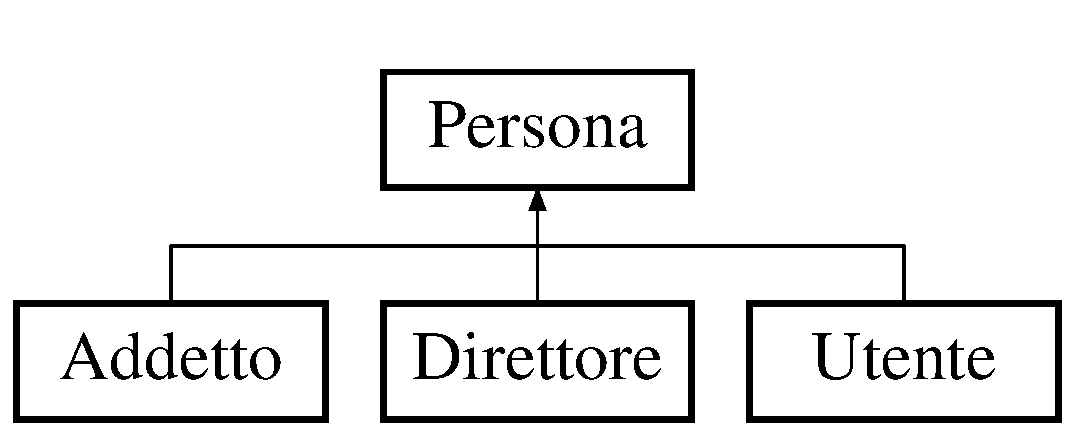
\includegraphics[height=2.000000cm]{class_persona}
\end{center}
\end{figure}
\subsection*{Membri pubblici}
\begin{DoxyCompactItemize}
\item 
\mbox{\hyperlink{class_persona_ac147ebfcfa0c66116e8ace9b53f91901}{Persona}} (char $\ast$, char $\ast$, char $\ast$)
\begin{DoxyCompactList}\small\item\em Costruttore \mbox{\hyperlink{class_persona}{Persona}}. \end{DoxyCompactList}\item 
\mbox{\Hypertarget{class_persona_aa7bba61c41b05166827eb1fbfc5ee0a9}\label{class_persona_aa7bba61c41b05166827eb1fbfc5ee0a9}} 
\mbox{\hyperlink{class_persona_aa7bba61c41b05166827eb1fbfc5ee0a9}{$\sim$\+Persona}} ()
\begin{DoxyCompactList}\small\item\em Distruttore \mbox{\hyperlink{class_persona}{Persona}}. \end{DoxyCompactList}\item 
void \mbox{\hyperlink{class_persona_a619e90d3b2036e78778b590ea1d51bcc}{Set\+Credenziali}} (char $\ast$, char $\ast$, char $\ast$)
\begin{DoxyCompactList}\small\item\em Setter delle credenziali. \end{DoxyCompactList}\item 
void \mbox{\hyperlink{class_persona_aa3d04ab73400a071421c979e692f93b3}{View\+Lista\+Prestiti}} ()
\begin{DoxyCompactList}\small\item\em Visualizzatore della Lista Prestiti. \end{DoxyCompactList}\item 
void \mbox{\hyperlink{class_persona_a8d7f6fa850c62e1eaac15c64013367a9}{View\+Lista\+Prestiti\+In\+Corso}} (char $\ast$username=\char`\"{}none\char`\"{})
\begin{DoxyCompactList}\small\item\em Visualizzatore della Lista Prestiti In Corso. \end{DoxyCompactList}\item 
void \mbox{\hyperlink{class_persona_ade5bba69999d1ccedd4104f1c6c323b6}{View\+Lista\+Prestiti\+Scaduti}} ()
\begin{DoxyCompactList}\small\item\em Visualizzatore della Lista Prestiti Scaduti. \end{DoxyCompactList}\item 
void \mbox{\hyperlink{class_persona_ad84db334efe5f35da14f085eec7383ce}{View\+Lista\+Utenti}} ()
\begin{DoxyCompactList}\small\item\em Visualizzatore della Lista Utenti. \end{DoxyCompactList}\item 
bool \mbox{\hyperlink{class_persona_ab06e2688ff0eb5c51177a44d33232070}{Ricerca\+Prestito}} (int $\ast$vett=new int\mbox{[}1000\mbox{]})
\begin{DoxyCompactList}\small\item\em Ricercatore del \mbox{\hyperlink{class_prestito}{Prestito}}. \end{DoxyCompactList}\item 
bool \mbox{\hyperlink{class_persona_a11bc0159627eb83be83b00c56ff1a3f9}{Ricerca\+Utente}} (int $\ast$vett=new int\mbox{[}1000\mbox{]})
\begin{DoxyCompactList}\small\item\em Ricercatore del \mbox{\hyperlink{class_prestito}{Prestito}}. \end{DoxyCompactList}\item 
void \mbox{\hyperlink{class_persona_ad46f21f01f3c49c7de0bb5bb0fca0251}{Registrazione\+Utente}} ()
\begin{DoxyCompactList}\small\item\em Registratore dell\textquotesingle{}\mbox{\hyperlink{class_utente}{Utente}}. \end{DoxyCompactList}\item 
void \mbox{\hyperlink{class_persona_a2da81a9fb38cf71e51a67efdb3510b13}{Modifica\+Libro}} ()
\begin{DoxyCompactList}\small\item\em Modificatore del \mbox{\hyperlink{class_libro}{Libro}}. \end{DoxyCompactList}\item 
void \mbox{\hyperlink{class_persona_aba5185684ebc81901b47abd587d01465}{Modifica\+Utente}} ()
\begin{DoxyCompactList}\small\item\em Modificatore dell\textquotesingle{}\mbox{\hyperlink{class_utente}{Utente}}. \end{DoxyCompactList}\item 
\mbox{\Hypertarget{class_persona_a49b4f6c55bf2cff47bb23478d6f160a1}\label{class_persona_a49b4f6c55bf2cff47bb23478d6f160a1}} 
void \mbox{\hyperlink{class_persona_a49b4f6c55bf2cff47bb23478d6f160a1}{Update\+Lista\+Prestiti}} (\mbox{\hyperlink{class_utente}{Utente}} $\ast$)
\begin{DoxyCompactList}\small\item\em Metodo per la modifica di Utenti in Lista Prestiti Richiesti. \end{DoxyCompactList}\item 
\mbox{\Hypertarget{class_persona_a163b75133201e6763d8dda84f9afa951}\label{class_persona_a163b75133201e6763d8dda84f9afa951}} 
void {\bfseries Update\+Lista\+Prestiti} (\mbox{\hyperlink{class_libro}{Libro}} $\ast$)
\item 
\mbox{\Hypertarget{class_persona_a5320069309eb9aff6c5da358b0c930c5}\label{class_persona_a5320069309eb9aff6c5da358b0c930c5}} 
void \mbox{\hyperlink{class_persona_a5320069309eb9aff6c5da358b0c930c5}{Update\+Lista\+Prestiti\+In\+Corso}} (\mbox{\hyperlink{class_utente}{Utente}} $\ast$)
\begin{DoxyCompactList}\small\item\em Metodo per la modifica di Utenti in Lista Prestiti In Corso. \end{DoxyCompactList}\item 
\mbox{\Hypertarget{class_persona_af08b858055be38620e154973efb215a0}\label{class_persona_af08b858055be38620e154973efb215a0}} 
void {\bfseries Update\+Lista\+Prestiti\+In\+Corso} (\mbox{\hyperlink{class_libro}{Libro}} $\ast$)
\item 
time\+\_\+t \mbox{\hyperlink{class_persona_a93d0e678c65154a03f07b0e5b48d6f78}{Get\+Data\+Registrazione}} ()
\begin{DoxyCompactList}\small\item\em Getter per la \mbox{\hyperlink{class_data}{Data}} di \mbox{\hyperlink{class_registrazione}{Registrazione}}. \end{DoxyCompactList}\item 
\mbox{\Hypertarget{class_persona_addab494a40e55af180c7b2e125bdc314}\label{class_persona_addab494a40e55af180c7b2e125bdc314}} 
void \mbox{\hyperlink{class_persona_addab494a40e55af180c7b2e125bdc314}{Set\+Data\+Registrazione}} ()
\begin{DoxyCompactList}\small\item\em Setter per la \mbox{\hyperlink{class_data}{Data}} di \mbox{\hyperlink{class_registrazione}{Registrazione}}. \end{DoxyCompactList}\item 
char $\ast$ \mbox{\hyperlink{class_persona_a840ce621ec4598d7c2c52cbfdf39764b}{Get\+Pin}} ()
\begin{DoxyCompactList}\small\item\em Getter per il \mbox{\hyperlink{class_pin}{Pin}}. \end{DoxyCompactList}\item 
char $\ast$ \mbox{\hyperlink{class_persona_a05788dcb627fed81b04c90a6b82121aa}{Get\+Nome}} ()
\begin{DoxyCompactList}\small\item\em Getter per il Nome. \end{DoxyCompactList}\item 
char $\ast$ \mbox{\hyperlink{class_persona_aac79de5438c101f8fa14a6c5011329b0}{Get\+Cognome}} ()
\begin{DoxyCompactList}\small\item\em Getter per il Cognome. \end{DoxyCompactList}\end{DoxyCompactItemize}


\subsection{Documentazione dei costruttori e dei distruttori}
\mbox{\Hypertarget{class_persona_ac147ebfcfa0c66116e8ace9b53f91901}\label{class_persona_ac147ebfcfa0c66116e8ace9b53f91901}} 
\index{Persona@{Persona}!Persona@{Persona}}
\index{Persona@{Persona}!Persona@{Persona}}
\subsubsection{\texorpdfstring{Persona()}{Persona()}}
{\footnotesize\ttfamily Persona\+::\+Persona (\begin{DoxyParamCaption}\item[{char $\ast$}]{pin,  }\item[{char $\ast$}]{nome,  }\item[{char $\ast$}]{cognome }\end{DoxyParamCaption})}



Costruttore \mbox{\hyperlink{class_persona}{Persona}}. 

Richiede 3 parametri in entrata\+: nome, cognome, pin. 

\subsection{Documentazione delle funzioni membro}
\mbox{\Hypertarget{class_persona_aac79de5438c101f8fa14a6c5011329b0}\label{class_persona_aac79de5438c101f8fa14a6c5011329b0}} 
\index{Persona@{Persona}!Get\+Cognome@{Get\+Cognome}}
\index{Get\+Cognome@{Get\+Cognome}!Persona@{Persona}}
\subsubsection{\texorpdfstring{Get\+Cognome()}{GetCognome()}}
{\footnotesize\ttfamily char $\ast$ Persona\+::\+Get\+Cognome (\begin{DoxyParamCaption}{ }\end{DoxyParamCaption})}



Getter per il Cognome. 


\begin{DoxyParams}[1]{Parametri}
\mbox{\tt out}  & {\em char$\ast$} & cognome \\
\hline
\end{DoxyParams}
\mbox{\Hypertarget{class_persona_a93d0e678c65154a03f07b0e5b48d6f78}\label{class_persona_a93d0e678c65154a03f07b0e5b48d6f78}} 
\index{Persona@{Persona}!Get\+Data\+Registrazione@{Get\+Data\+Registrazione}}
\index{Get\+Data\+Registrazione@{Get\+Data\+Registrazione}!Persona@{Persona}}
\subsubsection{\texorpdfstring{Get\+Data\+Registrazione()}{GetDataRegistrazione()}}
{\footnotesize\ttfamily time\+\_\+t Persona\+::\+Get\+Data\+Registrazione (\begin{DoxyParamCaption}{ }\end{DoxyParamCaption})}



Getter per la \mbox{\hyperlink{class_data}{Data}} di \mbox{\hyperlink{class_registrazione}{Registrazione}}. 


\begin{DoxyParams}[1]{Parametri}
\mbox{\tt out}  & {\em time\+\_\+t} & data\+Registrazione \\
\hline
\end{DoxyParams}
\mbox{\Hypertarget{class_persona_a05788dcb627fed81b04c90a6b82121aa}\label{class_persona_a05788dcb627fed81b04c90a6b82121aa}} 
\index{Persona@{Persona}!Get\+Nome@{Get\+Nome}}
\index{Get\+Nome@{Get\+Nome}!Persona@{Persona}}
\subsubsection{\texorpdfstring{Get\+Nome()}{GetNome()}}
{\footnotesize\ttfamily char $\ast$ Persona\+::\+Get\+Nome (\begin{DoxyParamCaption}{ }\end{DoxyParamCaption})}



Getter per il Nome. 


\begin{DoxyParams}[1]{Parametri}
\mbox{\tt out}  & {\em char$\ast$} & nome \\
\hline
\end{DoxyParams}
\mbox{\Hypertarget{class_persona_a840ce621ec4598d7c2c52cbfdf39764b}\label{class_persona_a840ce621ec4598d7c2c52cbfdf39764b}} 
\index{Persona@{Persona}!Get\+Pin@{Get\+Pin}}
\index{Get\+Pin@{Get\+Pin}!Persona@{Persona}}
\subsubsection{\texorpdfstring{Get\+Pin()}{GetPin()}}
{\footnotesize\ttfamily char $\ast$ Persona\+::\+Get\+Pin (\begin{DoxyParamCaption}{ }\end{DoxyParamCaption})}



Getter per il \mbox{\hyperlink{class_pin}{Pin}}. 


\begin{DoxyParams}[1]{Parametri}
\mbox{\tt out}  & {\em char$\ast$} & pin \\
\hline
\end{DoxyParams}
\mbox{\Hypertarget{class_persona_a2da81a9fb38cf71e51a67efdb3510b13}\label{class_persona_a2da81a9fb38cf71e51a67efdb3510b13}} 
\index{Persona@{Persona}!Modifica\+Libro@{Modifica\+Libro}}
\index{Modifica\+Libro@{Modifica\+Libro}!Persona@{Persona}}
\subsubsection{\texorpdfstring{Modifica\+Libro()}{ModificaLibro()}}
{\footnotesize\ttfamily void Persona\+::\+Modifica\+Libro (\begin{DoxyParamCaption}{ }\end{DoxyParamCaption})}



Modificatore del \mbox{\hyperlink{class_libro}{Libro}}. 

Richiamando la funzione Ricerca\+Libro() ne chiede la selezione del \mbox{\hyperlink{class_libro}{Libro}} e, una volta selezionato,~\newline
elenca i parametri che si vogliono modificare, a scelta tra Titolo, Autore, Anno, Codice.~\newline
La modifica avviene sia nel \mbox{\hyperlink{class_catalogo}{Catalogo}}, sia nella Lista Prestiti Scaduti, In Corso e Richiesti. \mbox{\Hypertarget{class_persona_aba5185684ebc81901b47abd587d01465}\label{class_persona_aba5185684ebc81901b47abd587d01465}} 
\index{Persona@{Persona}!Modifica\+Utente@{Modifica\+Utente}}
\index{Modifica\+Utente@{Modifica\+Utente}!Persona@{Persona}}
\subsubsection{\texorpdfstring{Modifica\+Utente()}{ModificaUtente()}}
{\footnotesize\ttfamily void Persona\+::\+Modifica\+Utente (\begin{DoxyParamCaption}{ }\end{DoxyParamCaption})}



Modificatore dell\textquotesingle{}\mbox{\hyperlink{class_utente}{Utente}}. 

Richiamando la funzione \mbox{\hyperlink{class_persona_a11bc0159627eb83be83b00c56ff1a3f9}{Ricerca\+Utente()}} ne chiede la selezione dell\textquotesingle{}\mbox{\hyperlink{class_utente}{Utente}} e, una volta selezionato,~\newline
elenca i parametri che si vogliono modificare, a scelta tra Nome, Cognome, \mbox{\hyperlink{class_pin}{Pin}}.~\newline
La modifica avviene sia nella Lista Utenti, sia nella Lista Prestiti Scaduti, In Corso e Richiesti. \mbox{\Hypertarget{class_persona_ad46f21f01f3c49c7de0bb5bb0fca0251}\label{class_persona_ad46f21f01f3c49c7de0bb5bb0fca0251}} 
\index{Persona@{Persona}!Registrazione\+Utente@{Registrazione\+Utente}}
\index{Registrazione\+Utente@{Registrazione\+Utente}!Persona@{Persona}}
\subsubsection{\texorpdfstring{Registrazione\+Utente()}{RegistrazioneUtente()}}
{\footnotesize\ttfamily void Persona\+::\+Registrazione\+Utente (\begin{DoxyParamCaption}{ }\end{DoxyParamCaption})}



Registratore dell\textquotesingle{}\mbox{\hyperlink{class_utente}{Utente}}. 

Richiede Nome, Cognome e Username da tastiera e fornisce il relativo \mbox{\hyperlink{class_pin}{Pin}} generato automaticamente. \mbox{\Hypertarget{class_persona_ab06e2688ff0eb5c51177a44d33232070}\label{class_persona_ab06e2688ff0eb5c51177a44d33232070}} 
\index{Persona@{Persona}!Ricerca\+Prestito@{Ricerca\+Prestito}}
\index{Ricerca\+Prestito@{Ricerca\+Prestito}!Persona@{Persona}}
\subsubsection{\texorpdfstring{Ricerca\+Prestito()}{RicercaPrestito()}}
{\footnotesize\ttfamily bool Persona\+::\+Ricerca\+Prestito (\begin{DoxyParamCaption}\item[{int $\ast$}]{vett = {\ttfamily new~int\mbox{[}1000\mbox{]}} }\end{DoxyParamCaption})}



Ricercatore del \mbox{\hyperlink{class_prestito}{Prestito}}. 


\begin{DoxyParams}[1]{Parametri}
\mbox{\tt out}  & {\em Conferma} & booleana presenza record in file.\\
\hline
\end{DoxyParams}
Richiede un testo in input, che varra\textquotesingle{} come parola chiave da ricercare in~\newline
Nome, Cognome \mbox{\hyperlink{class_utente}{Utente}}, Titolo, Autore, Anno, Codice \mbox{\hyperlink{class_libro}{Libro}}.~\newline
Restituisce, come indirizzo, un int$\ast$\mbox{[}1000\mbox{]} contenente gli indici dei singoli Prestiti trovati. \mbox{\Hypertarget{class_persona_a11bc0159627eb83be83b00c56ff1a3f9}\label{class_persona_a11bc0159627eb83be83b00c56ff1a3f9}} 
\index{Persona@{Persona}!Ricerca\+Utente@{Ricerca\+Utente}}
\index{Ricerca\+Utente@{Ricerca\+Utente}!Persona@{Persona}}
\subsubsection{\texorpdfstring{Ricerca\+Utente()}{RicercaUtente()}}
{\footnotesize\ttfamily bool Persona\+::\+Ricerca\+Utente (\begin{DoxyParamCaption}\item[{int $\ast$}]{vett = {\ttfamily new~int\mbox{[}1000\mbox{]}} }\end{DoxyParamCaption})}



Ricercatore del \mbox{\hyperlink{class_prestito}{Prestito}}. 


\begin{DoxyParams}[1]{Parametri}
\mbox{\tt out}  & {\em Conferma} & booleana presenza record in file.\\
\hline
\end{DoxyParams}
Richiede un testo in input, che varra\textquotesingle{} come parola chiave da ricercare in Nome, Cognome, \mbox{\hyperlink{class_pin}{Pin}}.~\newline
Restituisce, come indirizzo, un int$\ast$\mbox{[}1000\mbox{]} contenente gli indici dei singoli Utenti trovati. \mbox{\Hypertarget{class_persona_a619e90d3b2036e78778b590ea1d51bcc}\label{class_persona_a619e90d3b2036e78778b590ea1d51bcc}} 
\index{Persona@{Persona}!Set\+Credenziali@{Set\+Credenziali}}
\index{Set\+Credenziali@{Set\+Credenziali}!Persona@{Persona}}
\subsubsection{\texorpdfstring{Set\+Credenziali()}{SetCredenziali()}}
{\footnotesize\ttfamily void Persona\+::\+Set\+Credenziali (\begin{DoxyParamCaption}\item[{char $\ast$}]{pin,  }\item[{char $\ast$}]{nome,  }\item[{char $\ast$}]{cognome }\end{DoxyParamCaption})}



Setter delle credenziali. 

Funge da metodo setter per i 3 parametri\+: Nome, Cognome, \mbox{\hyperlink{class_pin}{Pin}}. \mbox{\Hypertarget{class_persona_aa3d04ab73400a071421c979e692f93b3}\label{class_persona_aa3d04ab73400a071421c979e692f93b3}} 
\index{Persona@{Persona}!View\+Lista\+Prestiti@{View\+Lista\+Prestiti}}
\index{View\+Lista\+Prestiti@{View\+Lista\+Prestiti}!Persona@{Persona}}
\subsubsection{\texorpdfstring{View\+Lista\+Prestiti()}{ViewListaPrestiti()}}
{\footnotesize\ttfamily void Persona\+::\+View\+Lista\+Prestiti (\begin{DoxyParamCaption}{ }\end{DoxyParamCaption})}



Visualizzatore della Lista Prestiti. 

Mostra il singolo prestito richiesto dall\textquotesingle{}\mbox{\hyperlink{class_utente}{Utente}} ne chiede l\textquotesingle{}accettazione da parte del relativo Addetto/\+Direttore. \mbox{\Hypertarget{class_persona_a8d7f6fa850c62e1eaac15c64013367a9}\label{class_persona_a8d7f6fa850c62e1eaac15c64013367a9}} 
\index{Persona@{Persona}!View\+Lista\+Prestiti\+In\+Corso@{View\+Lista\+Prestiti\+In\+Corso}}
\index{View\+Lista\+Prestiti\+In\+Corso@{View\+Lista\+Prestiti\+In\+Corso}!Persona@{Persona}}
\subsubsection{\texorpdfstring{View\+Lista\+Prestiti\+In\+Corso()}{ViewListaPrestitiInCorso()}}
{\footnotesize\ttfamily void Persona\+::\+View\+Lista\+Prestiti\+In\+Corso (\begin{DoxyParamCaption}\item[{char $\ast$}]{username = {\ttfamily \char`\"{}none\char`\"{}} }\end{DoxyParamCaption})}



Visualizzatore della Lista Prestiti In Corso. 

Mostra la lista dei prestiti in corso indicandone\+: Titolo \mbox{\hyperlink{class_libro}{Libro}}, Nome, Cognome, Username \mbox{\hyperlink{class_utente}{Utente}},~\newline
\mbox{\hyperlink{class_data}{Data}} Accettazione, \mbox{\hyperlink{class_data}{Data}} Scadenza, Giorni mancanti alla scadenza. \mbox{\Hypertarget{class_persona_ade5bba69999d1ccedd4104f1c6c323b6}\label{class_persona_ade5bba69999d1ccedd4104f1c6c323b6}} 
\index{Persona@{Persona}!View\+Lista\+Prestiti\+Scaduti@{View\+Lista\+Prestiti\+Scaduti}}
\index{View\+Lista\+Prestiti\+Scaduti@{View\+Lista\+Prestiti\+Scaduti}!Persona@{Persona}}
\subsubsection{\texorpdfstring{View\+Lista\+Prestiti\+Scaduti()}{ViewListaPrestitiScaduti()}}
{\footnotesize\ttfamily void Persona\+::\+View\+Lista\+Prestiti\+Scaduti (\begin{DoxyParamCaption}{ }\end{DoxyParamCaption})}



Visualizzatore della Lista Prestiti Scaduti. 

Mostra il singolo prestito scaduto e ne chiede la conferma del reso da parte del relativo Addetto/\+Direttore. \mbox{\Hypertarget{class_persona_ad84db334efe5f35da14f085eec7383ce}\label{class_persona_ad84db334efe5f35da14f085eec7383ce}} 
\index{Persona@{Persona}!View\+Lista\+Utenti@{View\+Lista\+Utenti}}
\index{View\+Lista\+Utenti@{View\+Lista\+Utenti}!Persona@{Persona}}
\subsubsection{\texorpdfstring{View\+Lista\+Utenti()}{ViewListaUtenti()}}
{\footnotesize\ttfamily void Persona\+::\+View\+Lista\+Utenti (\begin{DoxyParamCaption}{ }\end{DoxyParamCaption})}



Visualizzatore della Lista Utenti. 

Mostra la lista degli Utenti indicandone\+: Nome, Cognome, Username, \mbox{\hyperlink{class_pin}{Pin}}, \mbox{\hyperlink{class_data}{Data}} \mbox{\hyperlink{class_registrazione}{Registrazione}}. 

La documentazione per questa classe è stata generata a partire dai seguenti file\+:\begin{DoxyCompactItemize}
\item 
\mbox{\hyperlink{classi_8h}{classi.\+h}}\item 
\mbox{\hyperlink{funzioni_8cpp}{funzioni.\+cpp}}\end{DoxyCompactItemize}

\hypertarget{class_pin}{}\section{Riferimenti per la classe Pin}
\label{class_pin}\index{Pin@{Pin}}
\subsection*{Membri pubblici}
\begin{DoxyCompactItemize}
\item 
\mbox{\Hypertarget{class_pin_a462c14c45d3d653731dde638aa6e7bb7}\label{class_pin_a462c14c45d3d653731dde638aa6e7bb7}} 
\mbox{\hyperlink{class_pin_a462c14c45d3d653731dde638aa6e7bb7}{$\sim$\+Pin}} ()
\begin{DoxyCompactList}\small\item\em Distruttore \mbox{\hyperlink{class_pin}{Pin}}. \end{DoxyCompactList}\item 
char $\ast$ \mbox{\hyperlink{class_pin_a9295afd45c8d2a7ac6c73dfb528c2fd2}{Get\+Pin}} ()
\begin{DoxyCompactList}\small\item\em Getter per il nuovo \mbox{\hyperlink{class_pin}{Pin}} generato. \end{DoxyCompactList}\end{DoxyCompactItemize}


\subsection{Documentazione delle funzioni membro}
\mbox{\Hypertarget{class_pin_a9295afd45c8d2a7ac6c73dfb528c2fd2}\label{class_pin_a9295afd45c8d2a7ac6c73dfb528c2fd2}} 
\index{Pin@{Pin}!Get\+Pin@{Get\+Pin}}
\index{Get\+Pin@{Get\+Pin}!Pin@{Pin}}
\subsubsection{\texorpdfstring{Get\+Pin()}{GetPin()}}
{\footnotesize\ttfamily char $\ast$ Pin\+::\+Get\+Pin (\begin{DoxyParamCaption}{ }\end{DoxyParamCaption})}



Getter per il nuovo \mbox{\hyperlink{class_pin}{Pin}} generato. 


\begin{DoxyParams}[1]{Parametri}
\mbox{\tt out}  & {\em char$\ast$} & pin\\
\hline
\end{DoxyParams}
Restutuisce un pin generato pseudocausalmente covertito in char$\ast$, compreso tra 999 e 2000, estremi esclusi. 

La documentazione per questa classe è stata generata a partire dai seguenti file\+:\begin{DoxyCompactItemize}
\item 
\mbox{\hyperlink{classi_8h}{classi.\+h}}\item 
\mbox{\hyperlink{funzioni_8cpp}{funzioni.\+cpp}}\end{DoxyCompactItemize}

\hypertarget{class_prestito}{}\section{Riferimenti per la classe Prestito}
\label{class_prestito}\index{Prestito@{Prestito}}
\subsection*{Membri pubblici}
\begin{DoxyCompactItemize}
\item 
\mbox{\Hypertarget{class_prestito_a8052d0f665200b7a4cc232091e0599a7}\label{class_prestito_a8052d0f665200b7a4cc232091e0599a7}} 
\mbox{\hyperlink{class_prestito_a8052d0f665200b7a4cc232091e0599a7}{Prestito}} ()
\begin{DoxyCompactList}\small\item\em Costruttore \mbox{\hyperlink{class_prestito}{Prestito}}. \end{DoxyCompactList}\item 
\mbox{\Hypertarget{class_prestito_a470e008fe1b65ba194d2f06bb303c648}\label{class_prestito_a470e008fe1b65ba194d2f06bb303c648}} 
\mbox{\hyperlink{class_prestito_a470e008fe1b65ba194d2f06bb303c648}{$\sim$\+Prestito}} ()
\begin{DoxyCompactList}\small\item\em Distruttore \mbox{\hyperlink{class_prestito}{Prestito}}. \end{DoxyCompactList}\item 
\mbox{\Hypertarget{class_prestito_a8411d4f827e30d2d35ccb10886823e51}\label{class_prestito_a8411d4f827e30d2d35ccb10886823e51}} 
void \mbox{\hyperlink{class_prestito_a8411d4f827e30d2d35ccb10886823e51}{Set\+Data}} ()
\begin{DoxyCompactList}\small\item\em Setter \mbox{\hyperlink{class_data}{Data}} Accettazione e \mbox{\hyperlink{class_data}{Data}} Scadenza \mbox{\hyperlink{class_prestito}{Prestito}}. \end{DoxyCompactList}\item 
int \mbox{\hyperlink{class_prestito_a556664904743c53cc6504a913b0c7394}{Get\+Differenza}} ()
\begin{DoxyCompactList}\small\item\em Getter differenza tra \mbox{\hyperlink{class_data}{Data}} Scadenza e \mbox{\hyperlink{class_data}{Data}} Corrente. \end{DoxyCompactList}\item 
char $\ast$ \mbox{\hyperlink{class_prestito_ab7c954c58fe1a284c29af14acdf2a05f}{Get\+Codice}} ()
\begin{DoxyCompactList}\small\item\em Getter Codice del \mbox{\hyperlink{class_libro}{Libro}}. \end{DoxyCompactList}\item 
\mbox{\Hypertarget{class_prestito_a9cd58ea6672230249664e8453df67de9}\label{class_prestito_a9cd58ea6672230249664e8453df67de9}} 
void \mbox{\hyperlink{class_prestito_a9cd58ea6672230249664e8453df67de9}{Set\+Codice}} (char $\ast$)
\begin{DoxyCompactList}\small\item\em Setter Codice del \mbox{\hyperlink{class_libro}{Libro}}. \end{DoxyCompactList}\item 
time\+\_\+t \mbox{\hyperlink{class_prestito_afacba47375912f9d86b44cfae6bfd138}{Get\+Data\+Accettazione}} ()
\begin{DoxyCompactList}\small\item\em Getter \mbox{\hyperlink{class_data}{Data}} di Accettazione \mbox{\hyperlink{class_prestito}{Prestito}}. \end{DoxyCompactList}\item 
time\+\_\+t \mbox{\hyperlink{class_prestito_aefa87f49dcf99abf28ae20ebdb5f0325}{Get\+Data\+Scadenza}} ()
\begin{DoxyCompactList}\small\item\em Getter \mbox{\hyperlink{class_data}{Data}} di Scadenza \mbox{\hyperlink{class_prestito}{Prestito}}. \end{DoxyCompactList}\item 
\mbox{\Hypertarget{class_prestito_a8f4ddd024b8ffb5be270a190cb429ed9}\label{class_prestito_a8f4ddd024b8ffb5be270a190cb429ed9}} 
void \mbox{\hyperlink{class_prestito_a8f4ddd024b8ffb5be270a190cb429ed9}{Set\+Data\+Scadenza}} (time\+\_\+t)
\begin{DoxyCompactList}\small\item\em Setter \mbox{\hyperlink{class_data}{Data}} di Scadenza \mbox{\hyperlink{class_prestito}{Prestito}}. \end{DoxyCompactList}\end{DoxyCompactItemize}


\subsection{Documentazione delle funzioni membro}
\mbox{\Hypertarget{class_prestito_ab7c954c58fe1a284c29af14acdf2a05f}\label{class_prestito_ab7c954c58fe1a284c29af14acdf2a05f}} 
\index{Prestito@{Prestito}!Get\+Codice@{Get\+Codice}}
\index{Get\+Codice@{Get\+Codice}!Prestito@{Prestito}}
\subsubsection{\texorpdfstring{Get\+Codice()}{GetCodice()}}
{\footnotesize\ttfamily char $\ast$ Prestito\+::\+Get\+Codice (\begin{DoxyParamCaption}{ }\end{DoxyParamCaption})}



Getter Codice del \mbox{\hyperlink{class_libro}{Libro}}. 


\begin{DoxyParams}[1]{Parametri}
\mbox{\tt out}  & {\em char$\ast$} & codice\+Libro \\
\hline
\end{DoxyParams}
\mbox{\Hypertarget{class_prestito_afacba47375912f9d86b44cfae6bfd138}\label{class_prestito_afacba47375912f9d86b44cfae6bfd138}} 
\index{Prestito@{Prestito}!Get\+Data\+Accettazione@{Get\+Data\+Accettazione}}
\index{Get\+Data\+Accettazione@{Get\+Data\+Accettazione}!Prestito@{Prestito}}
\subsubsection{\texorpdfstring{Get\+Data\+Accettazione()}{GetDataAccettazione()}}
{\footnotesize\ttfamily time\+\_\+t Prestito\+::\+Get\+Data\+Accettazione (\begin{DoxyParamCaption}{ }\end{DoxyParamCaption})}



Getter \mbox{\hyperlink{class_data}{Data}} di Accettazione \mbox{\hyperlink{class_prestito}{Prestito}}. 


\begin{DoxyParams}[1]{Parametri}
\mbox{\tt out}  & {\em time\+\_\+t} & data\+Accettazione \\
\hline
\end{DoxyParams}
\mbox{\Hypertarget{class_prestito_aefa87f49dcf99abf28ae20ebdb5f0325}\label{class_prestito_aefa87f49dcf99abf28ae20ebdb5f0325}} 
\index{Prestito@{Prestito}!Get\+Data\+Scadenza@{Get\+Data\+Scadenza}}
\index{Get\+Data\+Scadenza@{Get\+Data\+Scadenza}!Prestito@{Prestito}}
\subsubsection{\texorpdfstring{Get\+Data\+Scadenza()}{GetDataScadenza()}}
{\footnotesize\ttfamily time\+\_\+t Prestito\+::\+Get\+Data\+Scadenza (\begin{DoxyParamCaption}{ }\end{DoxyParamCaption})}



Getter \mbox{\hyperlink{class_data}{Data}} di Scadenza \mbox{\hyperlink{class_prestito}{Prestito}}. 


\begin{DoxyParams}[1]{Parametri}
\mbox{\tt out}  & {\em time\+\_\+t} & data\+Scadenza \\
\hline
\end{DoxyParams}
\mbox{\Hypertarget{class_prestito_a556664904743c53cc6504a913b0c7394}\label{class_prestito_a556664904743c53cc6504a913b0c7394}} 
\index{Prestito@{Prestito}!Get\+Differenza@{Get\+Differenza}}
\index{Get\+Differenza@{Get\+Differenza}!Prestito@{Prestito}}
\subsubsection{\texorpdfstring{Get\+Differenza()}{GetDifferenza()}}
{\footnotesize\ttfamily int Prestito\+::\+Get\+Differenza (\begin{DoxyParamCaption}{ }\end{DoxyParamCaption})}



Getter differenza tra \mbox{\hyperlink{class_data}{Data}} Scadenza e \mbox{\hyperlink{class_data}{Data}} Corrente. 


\begin{DoxyParams}[1]{Parametri}
\mbox{\tt out}  & {\em Differenza} & in giorni \\
\hline
\end{DoxyParams}


La documentazione per questa classe è stata generata a partire dai seguenti file\+:\begin{DoxyCompactItemize}
\item 
\mbox{\hyperlink{classi_8h}{classi.\+h}}\item 
\mbox{\hyperlink{funzioni_8cpp}{funzioni.\+cpp}}\end{DoxyCompactItemize}

\hypertarget{class_registrazione}{}\section{Riferimenti per la classe Registrazione}
\label{class_registrazione}\index{Registrazione@{Registrazione}}
\subsection*{Membri pubblici}
\begin{DoxyCompactItemize}
\item 
\mbox{\Hypertarget{class_registrazione_a489e29298431ff6fef28de87ec06f986}\label{class_registrazione_a489e29298431ff6fef28de87ec06f986}} 
\mbox{\hyperlink{class_registrazione_a489e29298431ff6fef28de87ec06f986}{Registrazione}} ()
\begin{DoxyCompactList}\small\item\em Costruttore \mbox{\hyperlink{class_registrazione}{Registrazione}}. \end{DoxyCompactList}\item 
\mbox{\Hypertarget{class_registrazione_ac06a02bf41e1761459f78aab6ce6165f}\label{class_registrazione_ac06a02bf41e1761459f78aab6ce6165f}} 
\mbox{\hyperlink{class_registrazione_ac06a02bf41e1761459f78aab6ce6165f}{$\sim$\+Registrazione}} ()
\begin{DoxyCompactList}\small\item\em Distruttore \mbox{\hyperlink{class_registrazione}{Registrazione}}. \end{DoxyCompactList}\item 
void \mbox{\hyperlink{class_registrazione_a5fc942f14bcbc36267c23d95f7f4d833}{New\+Registrazione}} (char)
\begin{DoxyCompactList}\small\item\em Setter nuova \mbox{\hyperlink{class_registrazione}{Registrazione}}. \end{DoxyCompactList}\item 
char $\ast$ \mbox{\hyperlink{class_registrazione_aa74d88e1b4b3d4d8276fa52927b14428}{Get\+Nome}} ()
\begin{DoxyCompactList}\small\item\em Getter per il Nome. \end{DoxyCompactList}\item 
char $\ast$ \mbox{\hyperlink{class_registrazione_a3dfce4747c45ca52582848fd63fc6157}{Get\+Cognome}} ()
\begin{DoxyCompactList}\small\item\em Getter per il Cognome. \end{DoxyCompactList}\item 
char $\ast$ \mbox{\hyperlink{class_registrazione_aa330d25f3d6c56b14641bd3357d6c725}{Get\+Pin}} ()
\begin{DoxyCompactList}\small\item\em Getter per il \mbox{\hyperlink{class_pin}{Pin}}. \end{DoxyCompactList}\item 
char $\ast$ \mbox{\hyperlink{class_registrazione_a5e44252c4e10d35e1a8483fb6cccbef1}{Get\+Username}} ()
\begin{DoxyCompactList}\small\item\em Getter per l\textquotesingle{}Username. \end{DoxyCompactList}\item 
bool \mbox{\hyperlink{class_registrazione_acc22fb2c5ad3240e533125fd8701141e}{Get\+Is\+Registrato}} ()
\begin{DoxyCompactList}\small\item\em Getter per la conferma di \mbox{\hyperlink{class_registrazione}{Registrazione}}. \end{DoxyCompactList}\end{DoxyCompactItemize}


\subsection{Documentazione delle funzioni membro}
\mbox{\Hypertarget{class_registrazione_a3dfce4747c45ca52582848fd63fc6157}\label{class_registrazione_a3dfce4747c45ca52582848fd63fc6157}} 
\index{Registrazione@{Registrazione}!Get\+Cognome@{Get\+Cognome}}
\index{Get\+Cognome@{Get\+Cognome}!Registrazione@{Registrazione}}
\subsubsection{\texorpdfstring{Get\+Cognome()}{GetCognome()}}
{\footnotesize\ttfamily char $\ast$ Registrazione\+::\+Get\+Cognome (\begin{DoxyParamCaption}{ }\end{DoxyParamCaption})}



Getter per il Cognome. 


\begin{DoxyParams}[1]{Parametri}
\mbox{\tt out}  & {\em char$\ast$} & cognome \\
\hline
\end{DoxyParams}
\mbox{\Hypertarget{class_registrazione_acc22fb2c5ad3240e533125fd8701141e}\label{class_registrazione_acc22fb2c5ad3240e533125fd8701141e}} 
\index{Registrazione@{Registrazione}!Get\+Is\+Registrato@{Get\+Is\+Registrato}}
\index{Get\+Is\+Registrato@{Get\+Is\+Registrato}!Registrazione@{Registrazione}}
\subsubsection{\texorpdfstring{Get\+Is\+Registrato()}{GetIsRegistrato()}}
{\footnotesize\ttfamily bool Registrazione\+::\+Get\+Is\+Registrato (\begin{DoxyParamCaption}{ }\end{DoxyParamCaption})}



Getter per la conferma di \mbox{\hyperlink{class_registrazione}{Registrazione}}. 


\begin{DoxyParams}[1]{Parametri}
\mbox{\tt out}  & {\em bool} & is\+Registrato \\
\hline
\end{DoxyParams}
\mbox{\Hypertarget{class_registrazione_aa74d88e1b4b3d4d8276fa52927b14428}\label{class_registrazione_aa74d88e1b4b3d4d8276fa52927b14428}} 
\index{Registrazione@{Registrazione}!Get\+Nome@{Get\+Nome}}
\index{Get\+Nome@{Get\+Nome}!Registrazione@{Registrazione}}
\subsubsection{\texorpdfstring{Get\+Nome()}{GetNome()}}
{\footnotesize\ttfamily char $\ast$ Registrazione\+::\+Get\+Nome (\begin{DoxyParamCaption}{ }\end{DoxyParamCaption})}



Getter per il Nome. 


\begin{DoxyParams}[1]{Parametri}
\mbox{\tt out}  & {\em char$\ast$} & nome \\
\hline
\end{DoxyParams}
\mbox{\Hypertarget{class_registrazione_aa330d25f3d6c56b14641bd3357d6c725}\label{class_registrazione_aa330d25f3d6c56b14641bd3357d6c725}} 
\index{Registrazione@{Registrazione}!Get\+Pin@{Get\+Pin}}
\index{Get\+Pin@{Get\+Pin}!Registrazione@{Registrazione}}
\subsubsection{\texorpdfstring{Get\+Pin()}{GetPin()}}
{\footnotesize\ttfamily char $\ast$ Registrazione\+::\+Get\+Pin (\begin{DoxyParamCaption}{ }\end{DoxyParamCaption})}



Getter per il \mbox{\hyperlink{class_pin}{Pin}}. 


\begin{DoxyParams}[1]{Parametri}
\mbox{\tt out}  & {\em char$\ast$} & pin \\
\hline
\end{DoxyParams}
\mbox{\Hypertarget{class_registrazione_a5e44252c4e10d35e1a8483fb6cccbef1}\label{class_registrazione_a5e44252c4e10d35e1a8483fb6cccbef1}} 
\index{Registrazione@{Registrazione}!Get\+Username@{Get\+Username}}
\index{Get\+Username@{Get\+Username}!Registrazione@{Registrazione}}
\subsubsection{\texorpdfstring{Get\+Username()}{GetUsername()}}
{\footnotesize\ttfamily char $\ast$ Registrazione\+::\+Get\+Username (\begin{DoxyParamCaption}{ }\end{DoxyParamCaption})}



Getter per l\textquotesingle{}Username. 


\begin{DoxyParams}[1]{Parametri}
\mbox{\tt out}  & {\em char$\ast$} & username \\
\hline
\end{DoxyParams}
\mbox{\Hypertarget{class_registrazione_a5fc942f14bcbc36267c23d95f7f4d833}\label{class_registrazione_a5fc942f14bcbc36267c23d95f7f4d833}} 
\index{Registrazione@{Registrazione}!New\+Registrazione@{New\+Registrazione}}
\index{New\+Registrazione@{New\+Registrazione}!Registrazione@{Registrazione}}
\subsubsection{\texorpdfstring{New\+Registrazione()}{NewRegistrazione()}}
{\footnotesize\ttfamily void Registrazione\+::\+New\+Registrazione (\begin{DoxyParamCaption}\item[{char}]{registration\+Mode }\end{DoxyParamCaption})}



Setter nuova \mbox{\hyperlink{class_registrazione}{Registrazione}}. 

Come parametro di ingresso � richiesto un char (\textquotesingle{}u\textquotesingle{}\+:modalita\textquotesingle{} \mbox{\hyperlink{class_utente}{Utente}}, \textquotesingle{}a\textquotesingle{}\+:\mbox{\hyperlink{class_addetto}{Addetto}}, \textquotesingle{}d\textquotesingle{}\+:\mbox{\hyperlink{class_direttore}{Direttore}}).~\newline
Richiede Nome, Cognome e (se \mbox{\hyperlink{class_utente}{Utente}}) Username da tastiera e fornisce il relativo \mbox{\hyperlink{class_pin}{Pin}} generato automaticamente.~\newline
Le credenziali sono salvate in Credenziali Utenti/\+Addetti/\+Direttore. 

La documentazione per questa classe è stata generata a partire dai seguenti file\+:\begin{DoxyCompactItemize}
\item 
\mbox{\hyperlink{classi_8h}{classi.\+h}}\item 
\mbox{\hyperlink{funzioni_8cpp}{funzioni.\+cpp}}\end{DoxyCompactItemize}

\hypertarget{class_utente}{}\section{Riferimenti per la classe Utente}
\label{class_utente}\index{Utente@{Utente}}
Diagramma delle classi per Utente\begin{figure}[H]
\begin{center}
\leavevmode
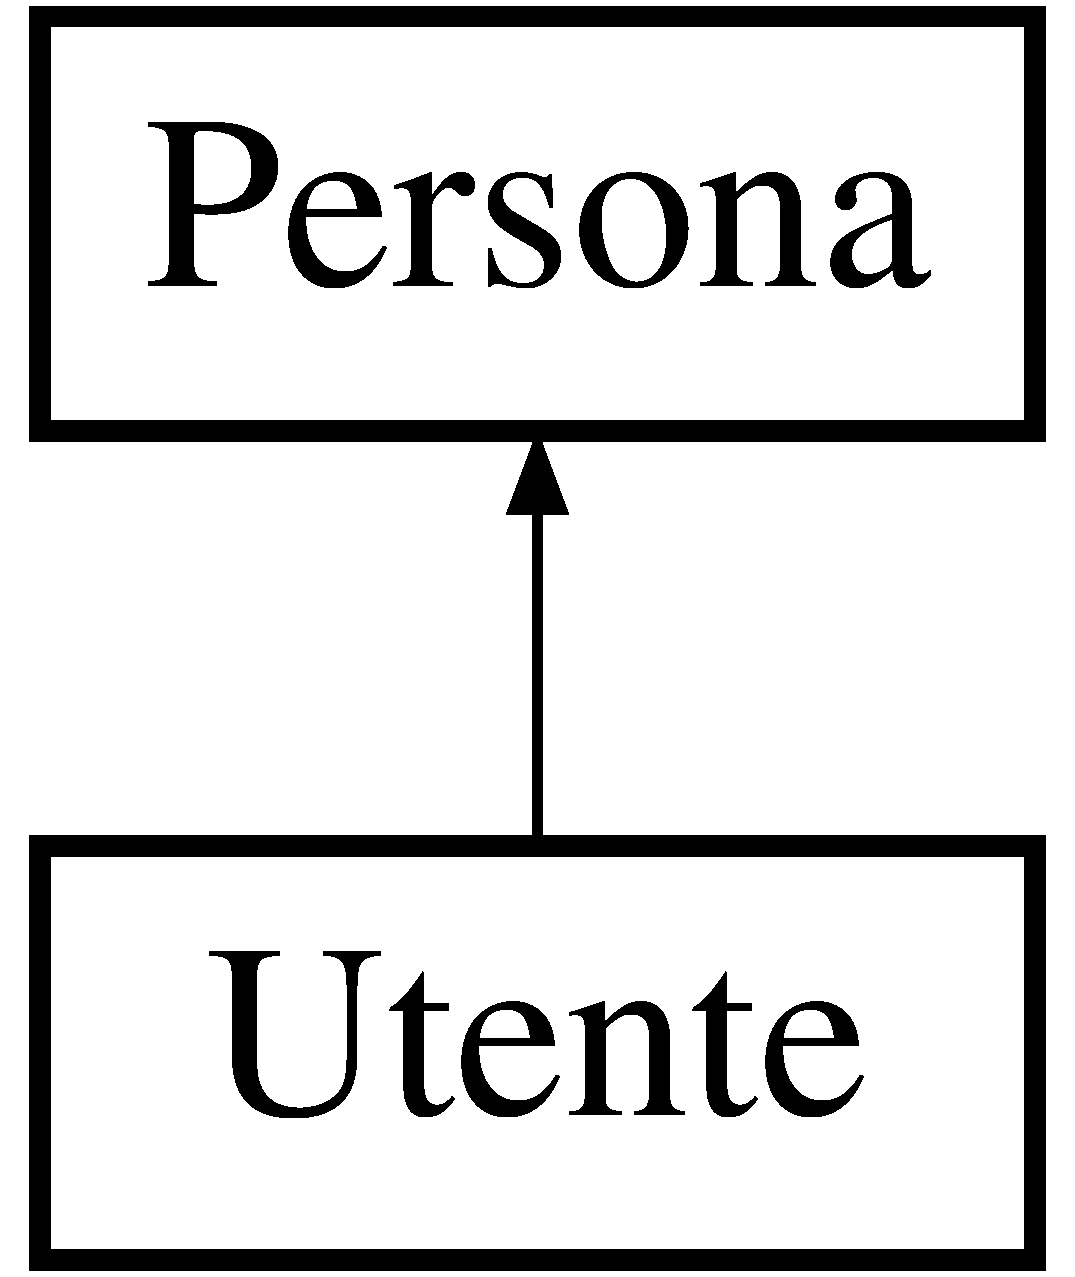
\includegraphics[height=2.000000cm]{class_utente}
\end{center}
\end{figure}
\subsection*{Membri pubblici}
\begin{DoxyCompactItemize}
\item 
\mbox{\Hypertarget{class_utente_ab1a579bcfe63412f3865c95c0b5802ee}\label{class_utente_ab1a579bcfe63412f3865c95c0b5802ee}} 
\mbox{\hyperlink{class_utente_ab1a579bcfe63412f3865c95c0b5802ee}{Utente}} (char $\ast$, char $\ast$, char $\ast$, char $\ast$)
\begin{DoxyCompactList}\small\item\em Costruttore \mbox{\hyperlink{class_utente}{Utente}}. \end{DoxyCompactList}\item 
\mbox{\Hypertarget{class_utente_a387f9b8358c4a8e99b9ce54332632ba5}\label{class_utente_a387f9b8358c4a8e99b9ce54332632ba5}} 
\mbox{\hyperlink{class_utente_a387f9b8358c4a8e99b9ce54332632ba5}{Utente}} ()
\begin{DoxyCompactList}\small\item\em Costruttore \mbox{\hyperlink{class_utente}{Utente}}. \end{DoxyCompactList}\item 
void \mbox{\hyperlink{class_utente_a6041323415b0cb311ab2564afdd6a13b}{Richiesta\+Prestito}} (\mbox{\hyperlink{class_utente}{Utente}} $\ast$)
\begin{DoxyCompactList}\small\item\em Richiesta \mbox{\hyperlink{class_prestito}{Prestito}} da parte dell\textquotesingle{}\mbox{\hyperlink{class_utente}{Utente}}. \end{DoxyCompactList}\item 
void \mbox{\hyperlink{class_utente_a42d4d04d073063464cf24d74723c0ba8}{Set\+User\+Credenziali}} (char $\ast$, char $\ast$, char $\ast$, char $\ast$)
\begin{DoxyCompactList}\small\item\em Setter delle credenziali dell\textquotesingle{}\mbox{\hyperlink{class_utente}{Utente}}. \end{DoxyCompactList}\item 
char $\ast$ \mbox{\hyperlink{class_utente_a9964d28e9b592fd7c430a55f09856727}{Get\+Username}} ()
\begin{DoxyCompactList}\small\item\em Getter per l\textquotesingle{}Username. \end{DoxyCompactList}\end{DoxyCompactItemize}


\subsection{Documentazione delle funzioni membro}
\mbox{\Hypertarget{class_utente_a9964d28e9b592fd7c430a55f09856727}\label{class_utente_a9964d28e9b592fd7c430a55f09856727}} 
\index{Utente@{Utente}!Get\+Username@{Get\+Username}}
\index{Get\+Username@{Get\+Username}!Utente@{Utente}}
\subsubsection{\texorpdfstring{Get\+Username()}{GetUsername()}}
{\footnotesize\ttfamily char $\ast$ Utente\+::\+Get\+Username (\begin{DoxyParamCaption}{ }\end{DoxyParamCaption})}



Getter per l\textquotesingle{}Username. 


\begin{DoxyParams}[1]{Parametri}
\mbox{\tt out}  & {\em char$\ast$} & username \\
\hline
\end{DoxyParams}
\mbox{\Hypertarget{class_utente_a6041323415b0cb311ab2564afdd6a13b}\label{class_utente_a6041323415b0cb311ab2564afdd6a13b}} 
\index{Utente@{Utente}!Richiesta\+Prestito@{Richiesta\+Prestito}}
\index{Richiesta\+Prestito@{Richiesta\+Prestito}!Utente@{Utente}}
\subsubsection{\texorpdfstring{Richiesta\+Prestito()}{RichiestaPrestito()}}
{\footnotesize\ttfamily void Utente\+::\+Richiesta\+Prestito (\begin{DoxyParamCaption}\item[{\mbox{\hyperlink{class_utente}{Utente}} $\ast$}]{u\+Pointer }\end{DoxyParamCaption})}



Richiesta \mbox{\hyperlink{class_prestito}{Prestito}} da parte dell\textquotesingle{}\mbox{\hyperlink{class_utente}{Utente}}. 

Richiamando la funzione Ricerca\+Libro() ne chiede la selezione del \mbox{\hyperlink{class_libro}{Libro}} e, una volta selezionato,~\newline
provvede ad inserire in Lista Prestiti Richiesti il \mbox{\hyperlink{class_prestito}{Prestito}} appena generato. \mbox{\Hypertarget{class_utente_a42d4d04d073063464cf24d74723c0ba8}\label{class_utente_a42d4d04d073063464cf24d74723c0ba8}} 
\index{Utente@{Utente}!Set\+User\+Credenziali@{Set\+User\+Credenziali}}
\index{Set\+User\+Credenziali@{Set\+User\+Credenziali}!Utente@{Utente}}
\subsubsection{\texorpdfstring{Set\+User\+Credenziali()}{SetUserCredenziali()}}
{\footnotesize\ttfamily void Utente\+::\+Set\+User\+Credenziali (\begin{DoxyParamCaption}\item[{char $\ast$}]{pin,  }\item[{char $\ast$}]{nome,  }\item[{char $\ast$}]{cognome,  }\item[{char $\ast$}]{username }\end{DoxyParamCaption})}



Setter delle credenziali dell\textquotesingle{}\mbox{\hyperlink{class_utente}{Utente}}. 

Funge da metodo setter per i 4 parametri\+: Nome, Cognome, \mbox{\hyperlink{class_pin}{Pin}}, Username. 

La documentazione per questa classe è stata generata a partire dai seguenti file\+:\begin{DoxyCompactItemize}
\item 
\mbox{\hyperlink{classi_8h}{classi.\+h}}\item 
\mbox{\hyperlink{funzioni_8cpp}{funzioni.\+cpp}}\end{DoxyCompactItemize}

\chapter{Documentazione dei file}
\hypertarget{classi_8h}{}\section{Riferimenti per il file classi.\+h}
\label{classi_8h}\index{classi.\+h@{classi.\+h}}


Header per la prototipazione delle classi.  


\subsection*{Composti}
\begin{DoxyCompactItemize}
\item 
class \mbox{\hyperlink{class_persona}{Persona}}
\item 
class \mbox{\hyperlink{class_direttore}{Direttore}}
\item 
class \mbox{\hyperlink{class_addetto}{Addetto}}
\item 
class \mbox{\hyperlink{class_utente}{Utente}}
\item 
class \mbox{\hyperlink{class_libro}{Libro}}
\item 
class \mbox{\hyperlink{class_catalogo}{Catalogo}}
\item 
class \mbox{\hyperlink{class_pin}{Pin}}
\item 
class \mbox{\hyperlink{class_registrazione}{Registrazione}}
\item 
class \mbox{\hyperlink{class_login}{Login}}
\item 
class \mbox{\hyperlink{class_data}{Data}}
\item 
class \mbox{\hyperlink{class_prestito}{Prestito}}
\end{DoxyCompactItemize}


\subsection{Descrizione dettagliata}
Header per la prototipazione delle classi. 

File di Prototipazione.

Racchiude l\textquotesingle{}intera struttura prototipata di ogni classe. 
\hypertarget{funzioni_8cpp}{}\section{Riferimenti per il file funzioni.\+cpp}
\label{funzioni_8cpp}\index{funzioni.\+cpp@{funzioni.\+cpp}}


Qua sono implementate tutte le funzioni.  


{\ttfamily \#include $<$iostream$>$}\newline
{\ttfamily \#include $<$string.\+h$>$}\newline
{\ttfamily \#include $<$fstream$>$}\newline
{\ttfamily \#include $<$time.\+h$>$}\newline
{\ttfamily \#include $<$cstdlib$>$}\newline
{\ttfamily \#include \char`\"{}classi.\+h\char`\"{}}\newline


\subsection{Descrizione dettagliata}
Qua sono implementate tutte le funzioni. 


\hypertarget{main_8cpp}{}\section{Riferimenti per il file main.\+cpp}
\label{main_8cpp}\index{main.\+cpp@{main.\+cpp}}


Da qui parte il software.  


{\ttfamily \#include $<$iostream$>$}\newline
{\ttfamily \#include $<$string.\+h$>$}\newline
{\ttfamily \#include $<$fstream$>$}\newline
{\ttfamily \#include $<$ctime$>$}\newline
{\ttfamily \#include $<$Windows.\+h$>$}\newline
{\ttfamily \#include $<$M\+M\+System.\+h$>$}\newline
{\ttfamily \#include \char`\"{}classi.\+h\char`\"{}}\newline
\subsection*{Funzioni}
\begin{DoxyCompactItemize}
\item 
\mbox{\Hypertarget{main_8cpp_a1dcf82671004d20b11a1e27deff01482}\label{main_8cpp_a1dcf82671004d20b11a1e27deff01482}} 
void {\bfseries User\+Mode} ()
\item 
\mbox{\Hypertarget{main_8cpp_a52b17c539d1c284157d4b9a63aadd781}\label{main_8cpp_a52b17c539d1c284157d4b9a63aadd781}} 
void {\bfseries Agent\+Mode} ()
\item 
\mbox{\Hypertarget{main_8cpp_a1cce51946a990e1559a80c5f3dfb8002}\label{main_8cpp_a1cce51946a990e1559a80c5f3dfb8002}} 
void {\bfseries Director\+Mode} ()
\item 
\mbox{\Hypertarget{main_8cpp_ae66f6b31b5ad750f1fe042a706a4e3d4}\label{main_8cpp_ae66f6b31b5ad750f1fe042a706a4e3d4}} 
int {\bfseries main} ()
\end{DoxyCompactItemize}


\subsection{Descrizione dettagliata}
Da qui parte il software. 


%--- End generated contents ---

% Index
\backmatter
\newpage
\phantomsection
\clearemptydoublepage
\addcontentsline{toc}{chapter}{Indice}
\printindex

\end{document}
